\documentclass[12pt]{article}

\usepackage[utf8]{inputenc}
\usepackage{makeidx}

\makeindex
\let\oldemph\emph
\renewcommand{\emph}[1]{\index{#1}\oldemph{#1}}

\usepackage{amsmath, amssymb, amsthm}



\DeclareMathOperator{\End}{End}
\DeclareMathOperator{\Ker}{Ker}
\DeclareMathOperator{\Imm}{Im}
\DeclareMathOperator{\I}{Im}
\DeclareMathOperator{\Hom}{Hom}
\DeclareMathOperator{\op}{op}
\DeclareMathOperator{\Mat}{Mat}
\DeclareMathOperator{\Irr}{Irr}

\DeclareMathOperator{\Id}{Id}
\usepackage{hyperref}



\newtheoremstyle{theorem}% name
  {}%         Space above, empty = `usual value'
  {}%         Space below
  {\itshape}% Body font
  {}%         Indent amount (empty = no indent, \parindent = para indent)
  {\bfseries}% Thm head font
  {.}%        Punctuation after thm head
  {\newline}% Space after thm head: \newline = linebreak
     {\def\temp{#3}\ifx\temp\empty\thmnumber{#2 }\thmname{#1}\else\thmnumber{#2}\thmnote{ #3}\fi}%         Head spec

%         Thm head spec
\theoremstyle{theorem}
\newtheorem{thm}{Theorem}[section]
\newtheorem{prop}[thm]{Proposition}
\newtheorem{lem}[thm]{Lemma}
\newtheorem{cor}[thm]{Corollary}

\swapnumbers
\newtheoremstyle{definition}% name
  {}%         Space above, empty = `usual value'
  {}%         Space below
  {}% Body font
  {}%         Indent amount (empty = no indent, \parindent = para indent)
  {\bfseries}% Thm head font
  {.}%        Punctuation after thm head
  {\newline}% Space after thm head: \newline = linebreak
  {}%         Thm head spec

\theoremstyle{definition}
\newtheorem{defn}[thm]{Definition}
\newtheorem{example}[thm]{Example}
\theoremstyle{remark}
\newtheorem{remark}[thm]{Remark}

\usepackage{parskip}

\makeatletter
\renewenvironment{proof}[1][\proofname] {\par\pushQED{\qed}\normalfont\topsep6\p@\@plus6\p@\relax\trivlist\item[\hskip\labelsep\bfseries#1\@addpunct{.}]\mbox{}\\*}{\popQED\endtrivlist\@endpefalse}
\makeatother

%Fix if theorem starts with a list
\makeatletter
\def\itemfix{%
\if@inlabel
 \noindent \par\nobreak\vskip-\baselineskip\hrule\@height\z@
\fi}

\let\olditemize\itemize
\def\itemize{\itemfix\olditemize}
\makeatother

\makeatletter
\def\enumfix{%
\if@inlabel
 \noindent \par\nobreak\vskip-\baselineskip\hrule\@height\z@
\fi}
\let\oldenumerate\enumerate
\def\enumerate{\enumfix\oldenumerate}


\usepackage{tkz-graph}

\tikzset{EdgeStyle/.append style = {->}}
\tikzset{LabelStyle/.style= {draw,
fill = white,
text = black}}

\begin{document}

\tableofcontents
\clearpage

%Week 1
\section{9-10-2014}

\subsection{Measure Theory Chapter 6}


\begin{thm}[Problem 6.1a]
Consider on \(\Bbb{R}\) the family \(\Sigma \) of all Borel sets which are symmetric w.r.t. the origin. Show that \(\Sigma \) is a \(\sigma \)-algebra.
\end{thm}

\begin{proof}

\begin{enumerate}
  \item To show that \(\Bbb{R}\in \Sigma \), note that \(\Bbb{R}\) is a Borel set that is symmetric w.r.t. to the origin.
  \item To show that \(A\in \Sigma \Rightarrow A^c\in \Sigma \), it suffices to show that
\[
\forall x\in A:-x\in A \Longrightarrow  \forall y\in A^c:-y\in A^c,
\]
which is equivalent with showing that
\[
\forall x\in A:-x\in A \Longrightarrow \forall y\not\in A : -y\not\in A,
\]
which is equivalent with showing that
\[
\exists y\not\in A:-y\in A \Longrightarrow \exists x\in A:-x\not\in A.
\]
This last statement hold if we set \(x:=-y.\)
  \item Showing that \(\Sigma \) is stable under countable unions is equivalent with showing that
\[
(A_{j})_{j\in \Bbb{N}}\in \Sigma \  \Longrightarrow \  \bigcup _{j=1}^\infty A_{j}\in \Sigma .
\]
It suffices to show that
\[
\forall x_{j}\in A_{j}:-x_{j}\in A_{j}\  \Longrightarrow \  \forall x\in \bigcup _{j=1}^\infty A_{j} :-x\in \bigcup _{j=1}^\infty A_{j}.
\]
This holds: Let \(x\in \bigcup _{j=1}^\infty A_{j}\). Then for some \(j\in \Bbb{N}\) we have \(x\in A_{j}\). By hypothesis, \(-x\in A_{j}.\) But then \(-x\in \bigcup _{j=1}^\infty A_{j}.\)

\end{enumerate}
\end{proof}
%
%\begin{thm}[Problem 6.1b]
%Is it possible to extend a pre-measure \(\mu \) on \(\Sigma \) to a measure on %\(\mathcal{B}(\Bbb{R})\) ?
%\end{thm}

%\begin{proof}
%Given a borel set $B$, make it a symmetric, by for example, taking all positive %values of $B$, call it $B_{+}$ together with $-B_{+}$. But this doesn't seem %unique. Couldn't I also just send all non-symmetric sets to $0$ ?
%\end{proof}
\newpage
\begin{thm}[Problem 6.3i]
Show that non-void open sets in \(\Bbb{R}^n\) have always strictly positive Lebesgue measure.
\end{thm}

\begin{proof}
First recall that

\begin{enumerate}
  \item \(\displaystyle \lambda ^n[a,b)=\prod _{j=1}^n(b_{j}-a_{j})\)
  \item \(\lambda ^n\) is a pre-measure that can be extended to a measure on \(\mathcal{B}(\Bbb{R}^n)\).
  \item \(\lambda ^n\) is invariant under translations
  \item \(A\subseteq B \Longrightarrow  \mu (A)\leq \mu (B)\)
\end{enumerate}

Remember we can contain a ball \(B_\epsilon(x)\) in any non-empty open set \(U\). Hence, to show that \(\lambda ^n(U)>0\) for any non-empty open set \(U\), it suffices to show that \(\lambda ^n(B_\epsilon(x))>0\).

But as \(\lambda ^n\) is invariant under translations, it suffices to show that \(\lambda ^n(B_\epsilon(0))>0.\)

We have that \(\lambda ^n[\dot{\epsilon},\dot{\epsilon})>0\) for any \(\dot{\epsilon}>0.\) Hence, it suffices to show that there exists such an \(\dot{\epsilon}\) such that \([\dot{\epsilon},\dot{\epsilon})\subseteq B_\epsilon(0).\)

This holds: Let \(x\in [\dot{\epsilon},\dot{\epsilon}).\) Then \(|x_{j}|<2\dot{\epsilon}.\) Then \(x_{j}^2<4\dot{\epsilon}^{2}\). Then
\[
x_{1}^2+x_{2}^2+\cdots +x_{n}^2<4n\dot{\epsilon}^2.
\]
So if we set \(\dot{\epsilon}:=\frac{\epsilon}{2\sqrt n}\). Then
\[
x_{1}^2+x_{2}^2+\cdots +x_{n}^2<\epsilon.
\]
And \(x\in B_\epsilon(0).\)

\end{proof}

\begin{thm}[Problem 6.3ii]
Is 6.3i still true for closed sets ?
\end{thm}

\begin{proof}
No, take \(\{0\}\), then \(\lambda \{x\}=0.\)
\end{proof}

\begin{thm}[Problem 6.4ii]
Let \(H\subseteq \Bbb{R}^{2}\) be a hyperplane which is perpendicular to the \(x_{1}\)-direction (that is to say: \(H\) is a translate of the \(x_{2}\) axis). Show that

\begin{enumerate}
  \item \(H\in \mathcal{B}(\Bbb{R}^2)\)
  \item \(\lambda ^2(H)=0\)
\end{enumerate}

\end{thm}

\begin{proof}
\begin{enumerate}
  \item To show that \(H\in \mathcal{B}(\Bbb{R}^2)\), it suffices to show that \(H\) is writable as an intersection of countable half-open sets.
Note that:
\[
H:=\{y\}\times\Bbb{R}=\bigcap _{j\in \Bbb{N}} [y,y+1/j)\times\Bbb{R}
\]
  \item To show that \(\lambda ^2(H)=0,\) it suffices to show that
\[
\forall \epsilon>0: \lambda ^2(H)<\epsilon.
\]

Let \(\epsilon>0\). Note that for any positive sequence \((\epsilon_{n})\), we have that:
\begin{align*}
\lambda ^2(H)&=\lambda ^{2} (\{y\} \times\Bbb{R}) \\
&\leq \lambda ^2\bigg(\bigcup _{n\in \Bbb{N}}[y,y+\epsilon_{n})\times[-n,n) \bigg)\\
&\leq \sum _{n=1}^\infty  \lambda ^2\Big([y,y+\epsilon_{n})\times[-n,n) \Big) \\
&=\sum _{n=1}^\infty \epsilon_{n} 2n.
\end{align*}
So if we set \(\epsilon_{n}:=\frac{\epsilon}{2^n2n}\). Then \(\lambda ^2(H)<\epsilon.\)
\end{enumerate}
\end{proof}
\newpage
\begin{thm}[Problem 6.4i]
Show that \(\lambda (a,b)=b-a\) for all \(a,b\in \Bbb{R},\space a\leq b\).
\end{thm}

\begin{proof}
\begin{align*}
\lambda (a,b) &=\lambda ([b-a)-\{b\}) \\
&=\lambda [b,a)-\lambda \{b\} &&\text{T4.3iii} \\
&=b-a-0 && \text{Problem 4.11i}
\end{align*}
\end{proof}

\begin{defn}
Let \((X,\mathcal{A},\mu )\) be a measure space such that all singletons \(\{x\}\in \mathcal{A}.\) A point \(x\) is called an atom, if \(\mu \{x\}>0.\) A measure is called \emph{non-atomic} or \emph{diffuse}, there are no atoms.
\end{defn}

\begin{thm}[Problem 6.5i]
Show that \(\lambda ^{1}\) is diffuse.
\end{thm}

\begin{proof}
We've already shown that \(\lambda \{x\}=0\) for any \(x\in \Bbb{R}\).
\end{proof}

\begin{thm}[Problem 6.5iii]
Show that for a diffuse measure \(\mu \) on \((X,\mathcal{A})\) all countable sets are null sets.
\end{thm}

\begin{proof}
All countable sets are writable as
\[
\bigcup _{j=0}^\infty \{x_{j}\}
\]
where \(x_{i}\neq x_{j}\). So we get
\[
\lambda \bigg(\bigcup _{j=0}^\infty \{x_{j}\}\bigg)=\sum _{j=0}^n\lambda \{x_{j}\}=0.
\]
\end{proof}

\begin{defn}
A set \(A\subseteq \Bbb{R}^n\) is called \emph{bounded} if it can be contained in a ball \(B_{r}\supseteq A\) of finite radius \(r\). A set \(A\subseteq \Bbb{R}^n\) is called \emph{connected}, if we can go along a curve from any point \(a\in A\) to any point \(a'\in A\) without ever leaving \(A\).
\end{defn}

\begin{thm}[Problem 6.6a]
Construct an open and unbounded set in \(\Bbb{R}\) with finite, strictly positive Lebesgue measure, i.e. \(0< \lambda(U)<\infty\).
\end{thm}

\begin{proof}
Consider the set
\[
U:=\bigcup _{n=1}^\infty  \bigg(n-\frac{1}{\epsilon_{n}},n+\frac{1}{\epsilon_{n}}\bigg).
\]

This is an open set, as it union of countable open sets. It is unbounded, for any \(B_{r}(0)\) we have that $\left \lceil {r+1}\right \rceil \in U$ and not in \(B_{r}(0)\). We have to show that it has positive finite lebesgue measure.
\begin{align*}
\lambda (U)&=\bigcup _{n=1}^\infty  \bigg(n-\frac{1}{\epsilon_{n}},n+\frac{1}{\epsilon_{n}}\bigg)\\
&=\sum _{n=1}^\infty \frac{2}{\epsilon_{n}}.
\end{align*}
So set \(\epsilon_{n}:=1/2^n.\) And we then have \(0<\lambda (U)=2<\infty .\)

\end{proof}

\begin{thm}[Problem 6.6ii]
Construct an open, unbounded and connected set in \(\Bbb{R}^2\) with finite, strictly positive Lebesgue measure.
\end{thm}

\begin{proof}
Let \((\epsilon_{n})\) be a positive sequence of real numbers. Consider
\[
U=\bigcup _{n=1}^\infty  (0,\epsilon_{n})\times(-n,n).
\]
This is an open set, as it is an countable union of open sets. It is clearly connected and unbounded in the \(y\)-axis. We now have that
then \begin{align*}
\lambda ^2(U)&=\bigg(\bigcup _{n\in \Bbb{N}}(0,\epsilon_{n})\times(-n,n) \bigg)\\
&\leq \sum _{n\in \Bbb{N}}\epsilon_{n}2n
\end{align*}
Set \(\epsilon_{n}:=\frac{1}{2^n2n}.\) Then \(\lambda ^2(U)=1\) is a positive finite real number.
\end{proof}

\begin{thm}[Problem 6.6iii]
Is there a connected, open and unbounded set in \(\Bbb{R}\) with finite, strictly positive Lebesgue measure ?
\end{thm}


\begin{proof}
No, this is impossible. Since we are in one dimension, connectedness forces us to go between points in a straight, uninterrupted line. Since the set is unbounded, this means we must have a line of the sort \((a,\infty )\) or \((-\infty ,b)\) in our set and in both cases Lebesgue measure is infinite.
\end{proof}

\begin{defn}
Let \(A \subset  X\). The closure of \(A\), denoted by \(\bar{A}\), is the smallest closed set
containing \(A\), i.e.

\[
\bar{A}=\bigcap_{\substack{F\in \mathcal{C}\\F\supset A}} F
\]

\end{defn}

\begin{defn}
A set \(A\subseteq X\) is dense in \(X\) if \(\bar{A}=X\)
\end{defn}

\begin{thm}[Problem 6.7]
Let \(\lambda :=\lambda ^1|_{[0,1]}\) be a Lebesgue measure on \(([0,1], \mathcal{B}[0,1])\). Show that for every \(\epsilon>0\) there is a dense open set \(U\subseteq [0,1]\) with \(\lambda (U)\leq \epsilon\).
\end{thm}

\begin{proof}
Note that \(\Bbb{Q}\) is dense. We are going to make an open set contained in \(\Bbb{Q}\).
Consider
\[
U:=\bigcup _{j=1}^\infty (q_{j}-\epsilon_{j},q_{j}+\epsilon_{j})
\]
Then
\[
\lambda (U)=\lambda (\bigcup _{j=1}^\infty (q_{j}-\epsilon_{j},q_{j}+\epsilon_{j}))\leq \sum 2\epsilon_{j}.
\]

So set \(\epsilon_{j}:=\frac{\epsilon}{2^{j-1}}\). And we are done.
\end{proof}

\begin{thm}[Problem 6.10i]
Let \(\mu \) be a measure on \(\mathcal{A}=\{\varnothing ,[0,1),[1,2),[0,2)\}\) of $X=[0,2)$. Such that
\[
\mu [0,1)=\mu [1,2)=1/2 \qquad \mu [0,2)=1.
\]

Define for each \(A\subseteq [0,2)\) the family of countable \(\mathcal{A}\)-coverings of \(A\)
\[
\mathcal{C}(A):=\{(A_{j})_{j\in \Bbb{N}}\subseteq \mathcal{A} : \bigcup _{j\in \Bbb{N}}A_{j} \supseteq A\}
\]
and set
\[
\mu ^*(A):=\inf\bigg\{\sum _{j\in \Bbb{N}}\mu (A_{j}) : (A_{j})_{j\in \Bbb{N}}\in \mathcal{C}(A)\bigg\}.
\]

Define \(\mathcal{A}^*:=\{A\subseteq [0,2): \mu ^*(B)=\mu ^*(B\cap A)+\mu ^*(B-A) \quad \forall B\subseteq X \}\)

Show that

\begin{enumerate}
  \item Find \(\mu ^*(a,b),\mu ^*\{a\}\)
  \item \((0,1),\{0\}\not\in \mathcal{A}^*\)
\end{enumerate}

\end{thm}

Note that in T6.1 it is proven that:

\begin{itemize}
  \item \(\mathcal{A}\subseteq \mathcal{A}^*\)
  \item \(\mu ^*(A)=\mu (A)  \quad \forall A\in \mathcal{A}\)
  \item \(\mathcal{A}^*\) is a \(\sigma \)-algebra and \(\mu ^*\) is a measure on \(([0,2),\mathcal{A}^*)\)
\end{itemize}
\newpage
\begin{proof}

\begin{enumerate}
  \item We have
\begin{align*}
\mu ^*(a,b)=\mu [0,1) \quad &\text{if } a,b\in [0,1)\\
\mu ^*(a,b)=\mu [1,2) \quad &\text{if } a,b\in [1,2)\\
\mu ^*(a,b)=\mu [0,2) \quad &\text{if } a\in [0,1),b\in [1,2)
\end{align*}
In the case of a singleton \(\{a\}\) the best posibble cover is always either \([0,1)\) or \([1,2)\) so that \(\mu ^*\{a\}=1/2.\)
  \item Suppose that \((0,1)\in \mathcal{A}^*\) then we would have that \[\{0\}=[0,1)-(0,1)\in \mathcal{A}^*.\] But this gives
\[
\frac{1}{2}=\mu ^*[0,1)=\mu ^*(0,1)+\mu ^*\{0\}=1
\]

\end{enumerate}

\end{proof}


\section{10-10-2014}
\subsection{Measure Theory Chapter 7}
\begin{defn}
Let \((X,\mathcal{A}),(X',\mathcal{A}')\) be two measurable spaces. A map \(T:X\rightarrow X'\) is called \emph{\(\mathcal{A}/\mathcal{A}'\)-measureable} (or \emph{measurable} unlesss this is too amiguous) if the pre-image of every measurable set is a measurable set:
\[
T^{-1}(A')\in \mathcal{A} \qquad \forall A'\in \mathcal{A}'.
\]
We often denote this by \(T^{-1}(\mathcal{A}')\subseteq \mathcal{A}'\).
\end{defn}

\begin{defn}
A \emph{random variable} is a measurable map from a probability space (i.e. \(\mu (X)=1)\) to any measurable space.
\end{defn}

\begin{thm}[Lemma 7.2]
Let \((X,\mathcal{A}),(X',\mathcal{A}')\) be measurable spaces and let \(\mathcal{A}'= \sigma (\mathcal{G}').\) Then \(T:X\rightarrow X'\) is \(\mathcal{A}/\mathcal{A}'\)-measurable if and only if
\[
T^{-1}(G')\in \mathcal{A} \qquad \forall G'\in \mathcal{G}'.
\]
\end{thm}

\begin{thm}[Problem 7.1]
Show that
\[
\tau _{x}:\Bbb{R}^n \rightarrow \Bbb{R}^n : B\mapsto B-x 
\]
is a \(\mathcal{B}(\Bbb{R}^n)/\mathcal{B}(\Bbb{R}^n)\) measurable map.
\end{thm}

\begin{proof}
Showing that
\[
\tau _{x}:\mathcal{B}(\Bbb{R}^n) \rightarrow \mathcal{B}(\Bbb{R}^n) : B\mapsto B-x
\]
is \(\mathcal{B}(\Bbb{R}^n)/\mathcal{B}(\Bbb{R}^n)\) measurable, is equivalent with showing that
\[
\tau _{x}^{-1}(B)\in \mathcal{B}(\Bbb{R}^n) \qquad \forall B\in \mathcal{B}(\Bbb{R}^n),
\]
which in turn is equivalent with showing that
\[
x+B\in \mathcal{B}(\Bbb{R}^n) \qquad \forall B\in \mathcal{J}(\Bbb{R}^n),
\]
which in turn is equivalent with showing that
\[
x+[a,b)\in \mathcal{B}(\Bbb{R}^n) \qquad \forall a,b\in \Bbb{R}^n.
\]
This follows as \(x+[a,b)=[x+a,x+b)\in \mathcal{J}(\Bbb{R}^n)\subseteq \mathcal{B}(\Bbb{R}^n).\)
\end{proof}

\begin{thm}
Every continuous map \(T:\Bbb{R}^n\rightarrow \Bbb{R}^m\) is \(\mathcal{B}^n/\mathcal{B}^m\) measurable.
\end{thm}

\begin{proof}
Showing that
\[
T:\Bbb{R}^n\rightarrow \Bbb{R}^m
\]
is \(\mathcal{B}^n/\mathcal{B}^m\) measurable, is equivalent with showing that
\[
T^{-1}(\mathcal{O}^m)\subseteq \mathcal{B}^n.
\]
As \(\mathcal{O}^n\subseteq \sigma (\mathcal{O}^n)= \mathcal{B}^n\), it suffices to show that
\[
T^{-1}(\mathcal{O}^m)\subseteq \mathcal{O}^n,
\]
which follows from the continuity of \(T\).
\end{proof}

\begin{defn}
Let \((T_{i})_{i\in I}\) be arbitrarily many mappings \(T_{i}:X\rightarrow X_{i}\) from the same space \(X\) into measurable spaces \((X_{i},\mathcal{A}_{i})\). The smallest \(\sigma \)-algebra on \(X\) that makes all \(T_{i}\) simultaneously measurable is
\[
\sigma (T_{i}:i\in I):=\sigma \Big(\bigcup _{i\in I}T_{i}^{-1}(\mathcal{A}_{i})\Big).
\]
We say that \(\sigma (T_{i}:i\in I)\) is \emph{generated by the family \((T_{i})_{i\in I}\)}.
\end{defn}

\begin{thm}
Let \((X_{j},A_{j}),j=1,2,3\), be measurable spaces and \(T:X_{1}\rightarrow X_{2},S:X_{2}\rightarrow X_{3}\) be \(\mathcal{A}_{1}/\mathcal{A}_{2}-\) resp. \(\mathcal{A}_{2}/\mathcal{A}_{3}\)-measurable maps. Then \(S\circ T:X_{1}\rightarrow X_{3}\) is \(\mathcal{A}_{1}/\mathcal{A}_{3}\)-measurable.
\end{thm}
\newpage
\begin{thm}[Problem 7.4]
Let \(X\) be a set, \((X_{i},\mathcal{A}_{i}),\space i\in I\),be arbitrarily many measurable spaces, and \(T_{i}:X\rightarrow X_{i}\) be a family of maps. Show that a map \(f\) from a measurable space \((F,\mathcal{F})\) to \((X,\sigma (T_{i}:i\in I)\) is measurable if, and only if, all maps \(T_{i}\circ f\) are \(\mathcal{F}/\mathcal{A}_{i}\)-measurable.
\end{thm}

\begin{proof}[Proof of $\Longrightarrow$]
To show that all maps \(T_{i}\circ f\) are \(\mathcal{F}/\mathcal{A}_{i}\)-measurable, it suffices to show that \(T_{i}:X\rightarrow X_{i}\) is \(\sigma (T_{i}:i\in I)/\mathcal{A}_{i}\)-measurable and \(f:F\rightarrow X\) is \(\mathcal{F}/\sigma (T_{i}:i\in I)\)-measurable.

By hypothesis, is suffices to show that \(T_{i}:X\rightarrow X_{i}\) is \(\sigma (T_{i}:i\in I)/\mathcal{A}_{i}\)-measurable, which is equivalent with showing that
\[
T_{i}^{-1}(A_{i})\in \sigma (T_{i}:i\in I)\qquad \forall A_{i}\in \mathcal{A}_{i}.
\]
It suffices to assume \(A_{i}\in \mathcal{A}_{i}\) and show that
\[
T_{i}^{-1}(A_{i})\in \bigcup _{i\in I}T_{i}^{-1}(\mathcal{A}_{i}) \qquad \checkmark.
\]
\end{proof}

\begin{proof}[Proof of $\Longleftarrow$]
To show that a map \(f\) from a measurable space \((F,\mathcal{F})\) to \((X,\sigma (T_{i}:i\in I)\) is measurable, it suffices to show that
\[
f^{-1}(\bigcup _{i\in I}T_{i}^{-1}(\mathcal{A}_{i}))\subseteq \mathcal{F}
\]
To show this it suffices to show that
\[
\bigcup _{i\in I}f^{-1}(T_{i}^{-1}(\mathcal{A}_{i}))\subseteq \mathcal{F},
\]
to show this it suffices to show that
\[
f^{-1}(T_{i}^{-1}(\mathcal{A}_{i}))\subseteq \mathcal{F},
\]
to show this it suffices to show that
\[
(T_{i}\circ f)^{-1}(\mathcal{A}_{i})\subseteq \mathcal{F}.
\]
This follows by hypothesis.
\end{proof}

\begin{thm}[Problem 7.8]
Let \(T:X\rightarrow Y\) be any map. Show that
\[
T^{-1}(\sigma (\mathcal{G)})=\sigma (T^{-1}(\mathcal{G}))
\]
holds for arbitrary families of \(\mathcal{G}\) of subsets of \(Y\).
\end{thm}

\begin{proof}
To show that
\[
T^{-1}(\sigma (\mathcal{G}))=\sigma (T^{-1}(\mathcal{G}))
\]
it suffices to show:

\begin{enumerate}
  \item \(T^{-1}(\sigma (\mathcal{G)})\subseteq \sigma (T^{-1}(\mathcal{G}))\)
  \item \(\sigma (T^{-1}(\mathcal{G}))\subseteq T^{-1}(\sigma (\mathcal{G}))\)
\end{enumerate}

To show
\[
T^{-1}(\sigma (\mathcal{G}))\subseteq \sigma (T^{-1}(\mathcal{G})),
\]
it suffices to show that
\(T\) is \(\sigma (T^{-1}(\mathcal{G}))/\sigma (\mathcal{G})\) measurable.

To show that it suffices to show that
\[
T^{-1}(\mathcal{G})\subseteq \sigma (T^{-1}(\mathcal{G})) \qquad \checkmark.
\]

To show
\[
\sigma (T^{-1}(\mathcal{G}))\subseteq T^{-1}(\sigma (\mathcal{G})),
\]
it suffices to show that
\[
T^{-1}(\mathcal{G})\subseteq T^{-1}(\sigma (\mathcal{G})) \qquad \checkmark.
\]
\end{proof}

\subsection{Measure Theory Chapter 5}
\begin{defn}
A family \(\mathcal{D}\subseteq \mathcal{P}(X)\) is a \emph{Dynkin system} if
\begin{gather*}
X\in \mathcal{D} \\
D\in \mathcal{D}\space \Longrightarrow \space D^c\in \mathcal{D} \\
(D_{j})_{j\in \Bbb{N}}\subseteq \mathcal{D} \text{ pairwise disjoint }\space \Longrightarrow \space \bigcup _{j\in \Bbb{N}}D_{j}\in \mathcal{D}
\end{gather*}
\end{defn}

\begin{defn}
Let \(\mathcal{G}\subseteq \mathcal{P}(X).\) Then there is a smallest Dynkin system \(\delta (\mathcal{G})\) containing \(\mathcal{G}\). \(\delta (\mathcal{G})\) is called the \emph{Dynkin system generated by \(\mathcal{G}\)}.
\end{defn}

\begin{prop}
Show that
\[
\mathcal{G}\subseteq \delta (\mathcal{G})\subseteq \sigma (\mathcal{G}).
\]
\end{prop}

\begin{proof}
We have that \(\mathcal{G}\subseteq \sigma (\mathcal{G})\). And therefore \(\delta (\mathcal{G})\subseteq \delta (\sigma (\mathcal{G}))=\sigma (\mathcal{G}).\)
\end{proof}

\begin{thm}
A Dynkin system \(\mathcal{D}\) is a \(\sigma \)-algebra if, and only if, it is stable under finite intersections: \(D,E\in \mathcal{D}\space \Longrightarrow \space D\cap E\in \mathcal{D}\)
\end{thm}

\begin{proof}
It suffices to show that a \(\cap \)-stable Dynkin system is stable under countable unions. To show this, it suffices to show that given $(D_{j})_{j\in \Bbb{N}}\in \mathcal{D}$, we have
\[
D:=\bigcup _{j\in \Bbb{N}}D_{j}\in \mathcal{D}.
\]

Set \(E_{1}=D_{1}\in \mathcal{D}\). And \(E_{2}:=D_{2}\cap D_{1}^c.\) And \(E_{3}=D_{3}\cap D_{2}^c\cap D_{1}^c\). And so on. Then
\[
D=\bigcup _{j\in \Bbb{N}}E_{j}\in \mathcal{D}.
\]
\end{proof}

\begin{thm}
If \(\mathcal{G}\subseteq \mathcal{P}(X)\) is stable under finite intersections, then \(\delta (\mathcal{G})=\sigma (\mathcal{G}).\)
\end{thm}

\begin{proof}
It suffices to show that \(\sigma (\mathcal{G})\subseteq \delta (\mathcal{G})\). As \(\mathcal{G}\subseteq \delta (\mathcal{G})\) it suffices to show that \(\delta (\mathcal{G})\) is a \(\sigma \)-algebra. To show that \(\delta (\mathcal{G})\) is a \(\sigma \)-algebra, it suffices to show that \(\delta (\mathcal{G})\) is stable under finite intersections.

Fix \(D\in \delta (G)\). Consider \(\mathcal{D}_D:=\{Q\subseteq X : Q\cap D \in  \delta (\mathcal{G}) \}\). It suffices to show that \(\delta (\mathcal{G})\subseteq \mathcal{D}_D\). To show that it suffices to show that \(\mathcal{D}_D\) is a Dynkin system and that \(\mathcal{G}\subseteq \mathcal{D}_D\).

To show that \(\mathcal{G}\subseteq \mathcal{D}_D\), it suffices to show that
\[
G\cap D\in \delta (\mathcal{G}) \qquad \forall G\in \mathcal{G},
\]
to show that it suffices to show that
\[
\delta (\mathcal{G})\subseteq \mathcal{D}_G \qquad \forall G\in \mathcal{G},
\]
to show that it suffices to show that (as \(\mathcal{D}_G\) is a dynkin system)
\[
\mathcal{G}\subseteq \mathcal{D}_G \qquad \forall G\in \mathcal{G}.
\]
This follows from \(\mathcal{G}\subseteq \delta (\mathcal{G})\) and \(\mathcal{G}\) is $\cap $-stable.
\end{proof}

\begin{prop}
\[
A_{j}\uparrow A\space \Longrightarrow \space A_{j}\cap B\uparrow A\cap B
\]
\end{prop}

\begin{proof}
To show that
\[
A_{j}\uparrow A\space \Longrightarrow \space A_{j}\cap B\uparrow A\cap B,
\]
it suffices to show that
\[
A=\bigcup _{j}A_{j}\space \Longrightarrow \space A\cap B=\bigcup _{j}A_{j}\cap B,
\]
which is equivalent with showing that
\[
\bigg(\bigcup _{j}A_{j}\bigg)\cap B=\bigcup _{j}A_{j}\cap B \qquad \checkmark.
\]

\end{proof}

\begin{defn}
An \emph{exhausting sequence} \((A_{j})_{j\in \Bbb{N}}\subseteq \mathcal{A}\) is an increasing sequence of sets \(A_{1}\subseteq A_{2}\subseteq A_{3}\subseteq ...\) such that \(\bigcup _{j\in \Bbb{N}}A_{j}=X\).
\end{defn}
\newpage
\begin{thm}
Assume that \((X,\mathcal{A})\) is a measurable space and that \(\mathcal{A}=\sigma (\mathcal{G})\) is generated by a family \(\mathcal{G}\) such that

\begin{itemize}
  \item \(\mathcal{G}\) is stable under finite intersections \(G,H\in \mathcal{G}\space \Longrightarrow \space G\cap H\in \mathcal{G}\)
  \item there exists an exhausting sequence \((G_{j})_{j\in \Bbb{N}}\subseteq \mathcal{G}\) with \(G_{j}\uparrow X\)
\end{itemize}

Any two measure \(\mu ,\nu \) that coincide on \(\mathcal{G}\) and are finite for all members of the exhausting sequence \(\mu (G_{j})=\nu (G_{j})<\infty \), are equal on \(\mathcal{A}\), i.e.
\[
\mu (A)=\nu (A) \qquad \forall A\in \mathcal{A}.
\]
\end{thm}

\begin{proof}
Remember that for any increasing sequence \((A_{j})_{j\in \Bbb{N}}\subseteq \mathcal{A}\) with \(A_{j}\uparrow A\in \mathcal{A}\) we have
\[
\mu (A)=\lim_{j\in \infty }\mu (A_{j}).
\]
To show that
\[
\mu (A)=\nu (A) \qquad \forall A\in \mathcal{A}
\]
it suffices to show that (as \(G_{j}\cap A\uparrow X\cap A)\)
\[
\lim_{j\in \infty }\mu (G_{j}\cap A)=\lim_{j\in \infty }\mu (G_{j}\cap A) \qquad \forall A\in \mathcal{A}
\]
To show that it suffices to show that
\[
\mu (G_{j}\cap A)=\nu (G_{j}\cap A) \qquad \forall j\in \Bbb{N}, \quad \forall A\in \mathcal{A}.
\]

Consider \(\mathcal{D}_{j}:=\{A\in \mathcal{A} : \mu (G_{j}\cap A)=\nu (G_{j}\cap A)\}\). It suffices to show that \(\mathcal{A}\subseteq \mathcal{D}_{j}\), which is equivalent with showing \(\sigma (\mathcal{G})\subseteq \mathcal{D}_{j}\).

As \(\mathcal{G}\) is stable under finite intersections, it suffices to show that \(\delta (\mathcal{G})\subseteq \mathcal{D}_{j}.\)

As \(\mathcal{G}\) is stable under finite intersections and \(\mu (\mathcal{G})=\nu (\mathcal{G})\), we have that \(\mathcal{G}\subseteq D_{j}\) and therefore it suffices to show that \(\mathcal{D}_{j}\) is a Dynkin system.

Which you can check.
\end{proof}

\begin{thm}
The \(n\)-dimensional Lebesgue measure \(\lambda ^n\) is invariant under translations, i.e.
\[
\lambda ^n(x+B)=\lambda ^n(B) \qquad\forall x\in \Bbb{R}^n,\forall B\in \mathcal{B}(\Bbb{R}^n).
\]
\end{thm}

\begin{proof}
Set \(\nu (B):=\lambda ^n(x+B)\) for some fixed \(x\in \Bbb{R}^n\). It suffices to show that
\[
\lambda ^n(B)=\nu (B)\qquad B\in \mathcal{B}.
\]
To show that, it suffices to show that

\begin{enumerate}
  \item \(\mathcal{J}\) is \(\cap \)-stable $\quad \checkmark$
  \item \(\mathcal{J}\) admits an exhausting sequence
\begin{itemize}
  \item \([-j,j)\uparrow \Bbb{R}^n\) \(\quad \checkmark\)
\end{itemize}
  \item \(\lambda ^n|_\mathcal{J}=\nu |_\mathcal{J}\)
\begin{align*}
v([a,b))&=\lambda ^n[x+a,x+b) \\
&=\lambda ^n[a,b)
\end{align*}
  \item \(\nu \) is a measure on \(\mathcal{B}^n\)
\end{enumerate}

To show that \(\nu \) is a measure on \(\mathcal{B}^n\), it suffices to show that
\[
\nu (\bigcup _{j\in \Bbb{N}}B_{j})=\sum _{j\in \Bbb{N}}\nu (B_{j}),
\]
which is equivalent with
\[
\lambda ^n(x+\bigcup _{j\in \Bbb{N}}B_{j})=\sum _{j\in \Bbb{N}}\lambda ^n(x+B_{j}).
\]
It suffices to show
\[
B\in \mathcal{B}^n\space \Longrightarrow \space x+B\in \mathcal{B}^n.
\]

Which we have already proven.

\end{proof}

\begin{thm}
Let \((X,\mathcal{A}),(X,\mathcal{A}')\) be measurable spaces and \(T:X\rightarrow X'\) be an \(\mathcal{A}/\mathcal{A}'\) measurable map. For every measure \(\mu \) on \((X,\mathcal{A})\),
\[
\mu '(A'):=\mu (T^{-1}(A')), \qquad A'\in \mathcal{A}'.
\]
The measure \(\mu '\) is called the \emph{image measure} of \(\mu \) under \(T\) and is denoted by \(T\circ \mu \) or \(\mu \circ T^{-1}\).
\end{thm}

\subsection{Measure Theory Chapter 7}
\begin{thm}[Problem 7.7]
Use image measures to give a new proof of Problem 5.8, i.e. to show that
\[
\lambda ^n(t\cdot B)=t^n\lambda ^n(B) \qquad \forall B\in \mathcal{B}(\Bbb{R}^n),\forall t>0
\]
\end{thm}

\begin{proof}
Set \(\nu (B):=t^n\lambda ^n(B)\) for some fixed \(x\in \Bbb{R}^n\). It suffices to show that
\[
\lambda ^n(tB)=\nu (B)\qquad \forall B\in \mathcal{B}.
\]
To show that, it suffices to show that

\begin{enumerate}
  \item \(\mathcal{J}\) is \(\cap \)-stable $\quad \checkmark$
  \item \(\mathcal{J}\) admits an exhausting sequence
\begin{itemize}
  \item \([-j,j)\uparrow \Bbb{R}^n\) \(\quad \checkmark\)
\end{itemize}
  \item \(\lambda ^n|_\mathcal{J}=\nu |_\mathcal{J}\)
\begin{align*}
\nu ([a,b))&=\lambda ^n[ta,tb) \\
&=t^n\lambda ^n[a,b)
\end{align*}
  \item \(\nu \) is a measure on \(\mathcal{B}^n\) as it is a composition of the inverse of a  measurable map and a measure.
\end{enumerate}
\end{proof}





\section{11-10-2014}
\begin{defn}
Note that:
\(u^{-1}[a,\infty )=\{x\in X:u(x)\in [a,\infty )\}=\{x\in X:u(x)\geq a\}.\)
We define:
\[
\{u(x)\geq a\}=u^{-1}[a,\infty ).
\]
\end{defn}

\begin{thm}
Let \((X,\mathcal{A})\) be a measurable space. The function \(u:X\rightarrow \Bbb{R}\) is \(\mathcal{A}/\mathcal{B}\)-measurable if, and only if, one, hence all, of the following conditions hold

\begin{enumerate}
  \item \(\{u\geq a\}\in \mathcal{A} \qquad \forall a\in \Bbb{R}\)
  \item \(\{u>a\}\in \mathcal{A} \qquad \forall a\in \Bbb{R}\)
  \item \(\{u\leq a\}\in \mathcal{A} \qquad \forall a\in \Bbb{R}\)
  \item \(\{u<a\}\in \mathcal{A} \qquad \forall a\in \Bbb{R}\)
\end{enumerate}
\end{thm}


\begin{defn}
We define the \emph{extended real line \(\bar{\Bbb{R}}:=[-\infty ,\infty ]\)} with the following rules for all \(x\in \Bbb{R}\):
\begin{align*}
x+\infty =\infty +x=\infty  \qquad &x+-\infty =-\infty +x=-\infty  \\
\infty +\infty =\infty  \qquad &-\infty -\infty =-\infty 
\end{align*}
And for \(x\in (0,\infty ]:\)
\begin{align*}
\pm x\cdot \infty &=\infty \cdot \pm x=\pm \infty  \\
\pm x\cdot -\infty &=-\infty \cdot \pm x=\mp \infty  \\
0\cdot \pm \infty &=\pm \infty \cdot 0=0 \\
\frac{1}{\pm \infty }&=0
\end{align*}
\end{defn}

\begin{defn}
Functions which take values in \(\bar{\Bbb{R}}\) are called \emph{numerical functions}.
\end{defn}

\begin{defn}
The Borel \(\sigma \)-algebra \(\bar{\mathcal{B}}=\mathcal{B}(\bar{\Bbb{R}})\) is defined by:
\[
\bar{\mathcal{B}}:=\bigg\{B\cup S : B\in \mathcal{B}\space  \text{ and }\space S\in \Big\{\varnothing ,\{-\infty \},\{\infty \},\{-\infty ,\infty \}\Big\}\bigg\}
\]
\end{defn}

\begin{thm}
We have \(\mathcal{B}(\Bbb{R})=\Bbb{R}\cap \mathcal{B}(\bar{\Bbb{R}})\). Moreover \(\bar{\mathcal{B}}\) is generated by all sets of the form \([a,\infty ]\) or \((a,\infty ]\) or \([-\infty ,a)\) or \([-\infty ,a]\) where \(a\in \Bbb{R}\)
\end{thm}

\begin{defn}
Let \((X,\mathcal{A})\) be a measurable space. We write \(\mathcal{M}:=\mathcal{M}(\mathcal{A})\) and \(\mathcal{M}_{\bar{\Bbb{R}}}:=\mathcal{M}_{\bar{\Bbb{R}}}(\mathcal{A})\) for the families of real valued \(\mathcal{A}/\mathcal{B}\)-measurable and numerical \(\mathcal{A}/\bar{\mathcal{B}}\)-measurable functions on \(X\).
\end{defn}

\begin{defn}
A \emph{simple function} \(g:X\rightarrow \Bbb{R}\) on a measurable space \((X,\mathcal{A})\) is a function of the form
\[
g(x):=\sum _{j=1}^M y_{j}\mathbf{1}_{A_{j}}(x)
\]
with finitely many sets \(A_{1},\ldots ,A_{m}\in \mathcal{A}\) and \(y_{1},\ldots ,y_M\in \Bbb{R}\). The set of simple functions is denoted by \(\mathcal{E}\) or \(\mathcal{E}(\mathcal{A})\).

If the sets \(A_{1},\ldots ,A_M\) are mutally disjoint we call
\[
\sum _{j=0}^M y_{j}\mathbf{1}_{A_{j}}(x)
\]
with \(y_{0}:=0\) and \(A_{0}:=(A_{1}\cup \ldots \cup A_M)^c\) a \emph{standard representation} of \(g\). Caution, this representation is not unique.
\end{defn}

\begin{thm}
Let \((X,\mathcal{A})\) be a measurable space. Every \(\mathcal{A}/\bar{\mathcal{B}}\)-measurable numerical function \(u:X\rightarrow \bar{\Bbb{R}}\) is the pointwise limit of simple functions:
\[
u(x)=\lim_{j\rightarrow \infty }f_{j}(x)
\]
where \(f_{j}\in \mathcal{E}(\mathcal{A})\) and \(|f_{j}|\leq |u|.\)

If \(u\geq 0\), all \(f_{j}\) can be chosen to be positive and increasing towards \(u\) so that \(u=\sup_{j\in \Bbb{N}}f_{j}\).
\end{thm}

\begin{thm}
Let \((X,\mathcal{A})\) be a measurable space. If \(u_{j}:X\rightarrow \bar{\Bbb{R}}, j\in \Bbb{N}\) are measurable functions, then so are
\[
\sup_{j\in \Bbb{N}}u_{j} \quad \inf_{j\in \Bbb{N}}u_{j} \quad \limsup_{j\rightarrow \Bbb{N}}u_{j}\quad \liminf_{j\rightarrow \Bbb{N}}u_{j}
\]
and whenever it exists
\[
\lim_{j\rightarrow \infty }u_{j}.
\]
\end{thm}

\begin{thm}
Let \(u,v\) be \(\mathcal{A}/\bar{\mathcal{B}}\)-measurable functions. Then the functions
\[
u\pm v \quad uv\quad u\vee v:=\max\{u,v\}\quad u\wedge v:=\min\{u,v\}
\]
are \(\mathcal{A}/\bar{\mathcal{B}}\)-measurable (whenever they are defined).
\end{thm}

\begin{thm}
A function \(u\) is \(\mathcal{A}/\mathcal{B}\) measurable if, and only if, \(u^\pm \) are \(\mathcal{A}/\bar{\mathcal{B}}\) measurable.
\end{thm}

\begin{thm}
Let \(T:(X,\mathcal{A})\rightarrow (X',\mathcal{A}')\) be an \(\mathcal{A}/\mathcal{A}'\)-measurable map and let \(\sigma (T)\subseteq \mathcal{A}\) be the \(\sigma \)-algebra generated by \(T\). Then \(u=w(T)\) for some \(\mathcal{A}'/\bar{\mathcal{B}}\) measurable function \(w:X'\rightarrow \bar{\Bbb{R}}\) if and only if
\(u:X\rightarrow \bar{\Bbb{R}}\) is \(\sigma (T)/\bar{\mathcal{B}}\)-measurable.
\end{thm}

\begin{prop}
Let \((X,\mathcal{A})\) be a measurable space. We define the indicator function:
\[
1_A : X\rightarrow  \Bbb{R} : x\in A \mapsto 1 \quad  x\in X-A\mapsto 0
\]
Show that the indicator function is measurable if, and only if, \(A\in \mathcal{A}.\)
\end{prop}

\begin{proof}
To show that \(1_A\) is measurable, it suffices to show that
\[
1_A^{-1}(a,\infty )\in \mathcal{A}.
\]

Note that
\[
1_A^{-1}(a,\infty )=\{x\in X:1_A(x)\in (a,\infty )\}=\{1_A >a\}
\]
If \(a\geq 1\), then \(1_A^{-1}(a,\infty )=\varnothing \).

If \(a\in [0,1)\), then  \(1_A^{-1}(a,\infty )=A.\)

If \(a<0\), then \(1_A^{-1}(a,\infty )=X\).
\end{proof}

\begin{prop}
Let \(A_{1},\ldots ,A_M\in \mathcal{A}\) be mutally disjoint sets and \(y_{1},\ldots ,y_M\in \Bbb{R}\). Then the function
\[
g: X\rightarrow \Bbb{R} : x\mapsto \sum _{j=1}^M y_{j}1_{A_{j}}(x)
\]
is measurable.
\end{prop}

\begin{proof}
To show that \(g\) is measurable it suffices to show that
\[
\{g>a\}\in \mathcal{A}
\]
i.e.
\[
\Big\{x\in X:\sum _{j=1}^M y_{j}1_{A_{j}}(x)>a\Big\}=\bigcup _{j:y_{j}>a}A_{j}\in \mathcal{A}.
\]
\end{proof}

\begin{thm}[Problem 8.3i]
Let \((X,\mathcal{A})\) be a measurable space. Let \(f,g : X\rightarrow \Bbb{R}\) be measurable functions. Show that for every \(A\in \mathcal{A}\) the functions \(h(x):=f(x)\) if \(x\in A\) and $h(x):=g(x)$, if \(x\not\in A\), is measurable.
\end{thm}

\begin{proof}
Note that
\[
h(x):=1_A(x)f(x)+1_{A^c}(x)g(x).
\]

And remember that sums and products of measurable functions are again measurable.
\end{proof}

\begin{thm}[Problem 8.3ii]
Let \((f_{j})_{j\in \Bbb{N}}\) be a sequence of measurable functions and let \((A_{j})_{j\in \Bbb{N}}\subseteq \mathcal{A}\) such that \(\bigcup _{j\in \Bbb{N}}A_{j}=X.\) Suppose that \(f_{j}|_{A_{j}\cap A_{k}}=f_{k}|_{A_{j}\cap A_{k}}\) for all \(j,k\in \Bbb{N}\) and set \(f(x):=f_{j}(x)\) if \(x\in A_{j}\). Show that \(f:X\rightarrow \Bbb{R}\) is measurable.<br />
\end{thm}

\begin{proof}
We have that:
\[
f^{-1}(B)=\bigcup _{j\in \Bbb{N}}A_{j}\cap f^{-1}(B)=\bigcup _{j\in \Bbb{N}}A_{j}\cap f_{j}^{-1}(B)\in \mathcal{A}
\]
\end{proof}

\begin{thm}[Problem 8.4]
Let \((X,\mathcal{A})\) be a measurable space and let \(\mathcal{B}\subset \mathcal{A}\) be a sub-\(\sigma \)-algebra. Show that \(\mathcal{M}(\mathcal{B})\subset \mathcal{M}(\mathcal{A}).\)
\end{thm}

\begin{proof}
To show that
\[
\mathcal{M}(\mathcal{B})\subset \mathcal{M}(\mathcal{A})
\]
it suffices to show there exists a \(\mathcal{A}\)-measurable function that is not \(\mathcal{B}\)-measurable. By hypothesis, we have an element \(A\in \mathcal{A}\), that is not in \(\mathcal{B}\), i.e. \(A\not\in \mathcal{B}\). Since \(1_A\) is \(\mathcal{B}\)-measurable if, and only if, \(B\in \mathcal{B}\), we have find the \(\mathcal{A}\)-measurable function where we where looking for.
\end{proof}

\begin{thm}
Let \(u:\Bbb{R}\rightarrow \Bbb{R}\) be differentiable. Explain why \(u\) and \(u'=du/dx\) are measurable.
\end{thm}

\begin{proof}
If \(u\) is differentiable, it is continuous, hence measurable. Since \(u'\) exists, we can write it in the form
\[
u'(x)=\lim_{k\rightarrow \infty } \frac{u(x+1/k)-u(x)}{1/k}
\]
i.e. as limit of measurable functions. Thus, \(u'\) is also measurable.
\end{proof}

\begin{thm}[Problem 8.17]
Show that the measurability of \(|u|\) does not, in general, imply the measurability of \(u\).
\end{thm}

\begin{proof}
Let \(A\subseteq \Bbb{R}\) be such that \(A\not\in \mathcal{B}\). Then it is clear that
\[
u(x):=1_A(x)-1_{A^c}(x)
\]
is not measurable. Take
\[
\{u=1\}=A\not\in \mathcal{A}.
\]
But \(|u(x)|=1\), which is a continuous function and therefore measurable.

\end{proof}

\begin{thm}[Problem 8.14]
Consider \((\Bbb{R},\mathcal{B})\) and \(u:\Bbb{R}\rightarrow \Bbb{R}\). Show that \(\{x\}\in \sigma (u)\) for all \(x\in \Bbb{R}\) if, and only if, \(u\) is injective.
\end{thm}

\begin{proof}
To show that \(u\) is injective, it suffices to assume $x,y\in \Bbb{R}$ and show that
\[
u(x)=u(y)\Longrightarrow x=y.
\]
Showing that is equivalent with showing that
\[
|\{u=u(x_{0})\}|=1.
\]
We surely have that \(\{x_{0}\}\subseteq \{u=u(x_{0})\}\). And note that
\[
\{x_{0}\}\in \sigma (u)=\sigma (u^{-1}(\mathcal{B}))
\]
just means that \(\{x_{0}\}=u^{-1}(B)\) for some $B\in \mathcal{B}$.
\end{proof}

\begin{proof}
Assume that \(u\) is injective,. This means that every point in the range \(u(\Bbb{R})\) comes exactly from unique defined \(x\in \Bbb{R}\). This can be expressed by saying that \(\{x\}=u^{-1}(\{u(x)\})=\{u(x)\}.\) But then
\[
\{x\}\in \sigma (u)=\sigma (u^{-1}(\mathcal{B})).
\]
\end{proof}


\section{12-10-2014}
\subsection{Measure Theory Chapter 9}
\begin{defn}
Let \(f=\sum _{j=0}^M y_{j}1_{A_{j}}\in \mathcal{E}^+\) be a simple function in standard representation. Then the number
\[
I_\mu (f):=\sum _{j=0}^My_{j}\mu (A_{j})\in [0,\infty ]
\]
is called the (\(\mu \)-)integral of \(f\).
\end{defn}

\begin{thm}

\begin{enumerate}
  \item \(I_\mu (1_A)=\mu (A) \qquad \forall A\in \mathcal{A}\)
  \item \(I_\mu (\lambda f)=\lambda I_\mu (f) \qquad \forall \lambda \geq 0\)
  \item \(I_\mu (f+g)=I_\mu (f)+I_\mu (g)\)
  \item \(f\leq g\space \Longrightarrow \space I_\mu (f)\leq I_\mu (g)\)

\end{enumerate}
\end{thm}

\begin{defn}
Let \((X,\mathcal{A},\mu )\) be a measure space. The (\(\mu \)-)integral of a positive numerical function \(u\in \mathcal{M}^+_{\bar{\Bbb{R}}}\) is given by
\[
\int  u d\mu :=\sup\{I_\mu (g) : g\leq u, g\in \mathcal{E}^+\}\in [0,\infty ].
\]
If we need to emphasize the integration variable, we also write
\[
\int u(x)\mu (dx)\quad \text{ or }\quad \int u(x)d\mu (x)
\]
\end{defn}

\begin{thm}
For all \(f\in \mathcal{E}^+\) we have \(\int fdu=I_\mu (f).\)
\end{thm}

\begin{thm}
Let \((X,A,\mu )\) be a measure space. For an increasing sequence of numerical functions \((u_{j})_{j\in \Bbb{N}}\subseteq \mathcal{M}^+_{\bar{\Bbb{R}}}, 0\leq u_{j}\leq u_{j+1}\leq \ldots \), we have \(u:=\sup_{j\in \Bbb{N}}u_{j}\in \mathcal{M}_{\bar{\Bbb{R}}}^+\) and
\[
\int \sup_{j\in \Bbb{N}}u_{j}d\mu  = \sup_{j\in \Bbb{N}} \int u_{j} d\mu 
\]
\end{thm}

\begin{thm}
Let \(u\in \mathcal{M}_{\bar{\Bbb{R}}}^+\). Then
\[
\int ud\mu  = \lim_{j\rightarrow \infty }\int f_{j}d\mu 
\]
holds for every increasing sequence \((f_{j})_{j\in \Bbb{N}}\subseteq \mathcal{E}^+\) with \(\lim_{j\rightarrow \infty }f_{j}=u\).
\end{thm}

\begin{thm}
Let \(u,v\in \mathcal{M}^+_{\bar{\Bbb{R}}}\). Then

\begin{enumerate}
  \item \(\int  1_A d\mu  = \mu (A) \quad \forall A\in \mathcal{A}\)
  \item \(\int  \alpha u d\mu  = \alpha  \int u d\mu \)
  \item \(\int (u+v)d\mu  = \int ud\mu  +\int vd\mu \)
  \item \(u\leq v\space \Longrightarrow \space \int ud\mu \leq \int vd\mu \)
\end{enumerate}
\end{thm}


\begin{thm}
Let \((u_{j})_{j\in \Bbb{N}}\subseteq \mathcal{M}^+_{\bar{\Bbb{R}}}\). Then \(\sum _{j=1}^\infty u_{j}\) is measurable and we have
\[
\int \sum _{j=1}^\infty u_{j}d\mu =\sum _{j=1}^\infty \int u_{j}d\mu 
\]
\end{thm}

\begin{thm}
Let \((u_{j})_{j\in \Bbb{N}}\subseteq \mathcal{M}^+_{\bar{\Bbb{R}}}\) be a sequence of positive measurable numerical functions. Then \(u:=\liminf_{j\in \infty }\int u_{j}d\mu \) is measurable and
\[
\int \liminf_{j\rightarrow \infty }u_{j}d\mu \leq \liminf_{j\rightarrow \infty }\int u_{j}d\mu 
\]
\end{thm}

\begin{thm}[Problem 9.1]
Let \(f:X\rightarrow \Bbb{R}\) be a positive simple function of the form
\[
f(x)=\sum _{j=1}^m \xi _{j}1_{A_{j}}(x)\qquad \xi _{j}\geq 0 , A_{j}\in \mathcal{A}.
\]
Show that
\[
I_\mu (f)=\sum _{j=1}^m\xi _{j}\mu (A_{j})
\]
\end{thm}

\begin{proof}
\[
I_\mu (f)=I_\mu \bigg(\sum _{j=1}^m \xi _{j}1_{A_{j}}\bigg)=\sum _{j=1}^m\xi _{j}I_\mu (1_{A_{j}})=\sum _{j=1}^m\xi _{j}\mu (A_{j})
\]
\end{proof}


\begin{thm}[Problem 9.5]
Let \((X,\mathcal{A},\mu )\) be a measure space and \(u\in \mathcal{M}^+(\mathcal{A})\). Show that the set-function
\[
A\mapsto \int 1_Aud\mu  \quad A\in \mathcal{A}
\]
is a measure.
\end{thm}

\begin{proof}
Set
\[
\nu :\mathcal{A}\rightarrow [0,\infty ]:A\mapsto \int 1_Aud\mu .
\]

\begin{enumerate}
  \item To show that \(\nu (\varnothing )=0\). Notice that \(1_\varnothing \equiv 0\).
  \item Let \(A=\bigcup _{j\in \Bbb{N}}A_{j}\) a disjoint union of sets \(A_{j}\in \mathcal{A}\). Note that
\[
\sum _{j=1}^\infty 1_{A_{j}}=1_A
\]
We have to show that
\begin{align*}
\nu (\bigcup _{j\in \Bbb{N}}A_{j})&=\int \bigg(\sum _{j=1}^\infty 1_{A_{j}}\bigg)\cdot ud\mu  \\
&=\int \bigg(\sum _{j=1}^\infty 1_{A_{j}}u\bigg)d\mu   \\
&= \sum _{j=1}^\infty \int 1_{A_{j}}ud\mu  \\
&= \sum _{j=1}^\infty  \nu (A_{j}).
\end{align*}
\end{enumerate}

\end{proof}



\begin{thm}[Problem 9.8]
Let \((X,\mathcal{A},\mu )\) be a measure space and \((u_{j})_{j\in \Bbb{N}}\subseteq \mathcal{M}^+(\mathcal{A}).\) If \(u_{j}\leq u\) for all \(j\in \Bbb{N}\) and some \(u\in \mathcal{M}^+(\mathcal{A})\) with \(\int ud\mu <\infty \), then
\[
\limsup_{j\in \infty }\int u_{j}d\mu \leq \int \limsup_{j\in \infty }u_{j}d\mu .
\]
\end{thm}

\begin{proof}
Showing that
\[
\limsup_{j\in \infty }\int u_{j}d\mu \leq \int \limsup_{j\in \infty }u_{j}d\mu 
\]
is equivalent with showing that
\[
-\liminf_{j\in \infty }\int -u_{j}d\mu \leq -\int \liminf_{j\in \infty }-u_{j}d\mu 
\]
which is equivalent with showing that
\[
\int \liminf_{j\in \infty }-u_{j}d\mu \leq \liminf_{j\in \infty }\int -u_{j}d\mu 
\]
which is equivalent with showing that
\[
\int ud\mu  + \int \liminf_{j\in \infty }-u_{j}d\mu \leq \int ud\mu  +\liminf_{j\in \infty }\int -u_{j}d\mu 
\]
which is equivalent with showing that
\[
\int u + \liminf_{j\in \infty }-u_{j}d\mu \leq \liminf_{j\in \infty }\bigg(\int ud\mu  +\int -u_{j}d\mu \bigg)
\]
which is equivalent with showing that
\[
\int  \liminf_{j\in \infty }\Big(u -u_{j}\Big)d\mu \leq \liminf_{j\in \infty }\bigg(\int u -u_{j}d\mu \bigg).
\]

By hypothesis, \(u_{j}\leq u\). So we have that \(u-u_{j}\) is a sequence of postive measurable functions and therefore our last statement follows by the theorem of Fatou.
\end{proof}
\newpage
\subsection{Measure Theory Chapter 7}

\begin{prop}
Let \((X,\mathcal{A}),(X',\mathcal{A}')\) be measurable spaces and let \(\mathcal{A}'=\sigma (\mathcal{G}').\) Then \(T:X\rightarrow X'\) is \(\mathcal{A}/\mathcal{A}'\)-measurable if and only if \(T^{-1}(\mathcal{G}')\subseteq \mathcal{A}.\)
\end{prop}

It suffices to show assume \(T^{-1}(\mathcal{G}')\subseteq \mathcal{A}\) and show that
\[
T^{-1}(\mathcal{A})\subseteq \mathcal{A}.
\]

Consider \(\Sigma :=\{A'\subseteq X' : T^{-1}(A')\in \mathcal{A}\}\). We have that \(\mathcal{G}'\subseteq \Sigma \). It suffices to show that
\[
\mathcal{A}'\subseteq \Sigma .
\]
It suffices to show that \(\Sigma \) is a \(\sigma \)-algebra.

\begin{enumerate}
  \item To show that \(X'\in \Sigma \), it suffices to show that \(T^{-1}(X')\in \mathcal{A}\).
  \item Showing that
\[
A'\in \Sigma  \Longrightarrow  A'^c\in \Sigma 
\]
is equivalent with showing that
\[
T^{-1}(A')\in \mathcal{A} \Longrightarrow  T^{-1}(A'^c)\in \mathcal{A} \qquad\checkmark
\]
  \item Showing that
\[
(A_{j}')_{j\in \Bbb{N}}\subseteq \Sigma  \Longrightarrow  \bigcup _{j\in \Bbb{N}}A_{j}\in \Sigma 
\]
is equivalent with showing that
\[
T^{-1}(A_{j}')\in \mathcal{A}\Longrightarrow T^{-1}\Big(\bigcup _{j\in \Bbb{N}}A_{j}\Big)\in \mathcal{A} \qquad\checkmark
\]
\end{enumerate}

\begin{prop}
Let \((X,\mathcal{A}),(X,\mathcal{A}')\) be measurable spaces and \(T:X\rightarrow X'\) be an \(\mathcal{A}/\mathcal{A}'\)-measurable map. For every measure \(\mu \) on \((X,\mathcal{A})\),
\[
\mu '(A'):=T(\mu )(A'):=\mu (T^{-1}(A')), \qquad A'\in \mathcal{A}'
\]
defines a measure on \((X',\mathcal{A}').\)
\end{prop}

\begin{proof}

\begin{enumerate}
  \item To show that
\[
\mu (T^{-1}(\varnothing ))=0 \qquad \checkmark
\]
  \item Assume \((A_{j}')_{j\in \Bbb{N}}\subseteq \mathcal{A}'\) mutually disjoint sets and show that
\[
\mu '(\bigcup _{j\in \Bbb{N}}A_{j}')=\sum _{j\in \Bbb{N}}\mu '(A_{j}'),
\]
which is equivalent with showing that
\[
\mu (T^{-1}\Big(\bigcup _{j\in \Bbb{N}}A_{j}'\Big)=\sum _{j\in \Bbb{N}}\mu (T^{-1}(A_{j}')),
\]
which is equivalent with showing that
\[
\mu (T^{-1}\Big(\bigcup _{j\in \Bbb{N}}A_{j}'\Big)=\mu \Big(\bigcup _{j\in \Bbb{N}}T^{-1}(A_{j}')\bigg) \qquad \checkmark.
\]
\end{enumerate}

\end{proof}
\begin{thm}[Problem 7.9i]
Let \(\mu \) be a measure on \((\Bbb{R},\mathcal{B})\). Show that
\[
F_\mu (x):=\begin{cases}\mu [0,x) &\text{ if }x>0 \\0 & \text{ if }x=0 \\ -\mu [x,0) &\text{ if }x<0\end{cases}
\]

\begin{enumerate}
  \item is monotonically increasing
  \item left-continuous funciton
\end{enumerate}
\end{thm}


\begin{proof}

\begin{enumerate}
  \item Showing that \(F_\mu \) is monotonically increasing is equivalent with showing that
\[
x\leq y \Longrightarrow  F_\mu (x)\leq F_\mu (y).
\]

\begin{enumerate}
  \item $x\leq 0\leq y:$. Then \(F_\mu (x)=-\mu [x,0)\leq 0\) and \(F_\mu (y)=\mu [0,y)\geq 0\).
  \item \(0<x\leq y:\) Then \([0,x)\subseteq [0,y)\). And \(\mu [0,x)\leq \mu [0,y)\).
  \item \(x\leq y<0:\) Then \([y,0)\subseteq [x,0).\) And \(\mu [y,0)\leq \mu [x,0)\).
\end{enumerate}
  \item Showing that \(F_\mu \) is left continuous is equivalent with assuming $(x_{k})$ a sequence such that \(x_{k}<x\) and \(x_{k}\uparrow x\) and showing that
\[
\lim_{k\rightarrow \infty }F_\mu (x_{k})=F_\mu (x).
\]
If if $x>0$, it suffices to show that
\[
\lim_{k\rightarrow \infty }\mu [0,x_{k})=\mu [0,x).
\]
If \(x<0\) it suffices to show that
\[
\lim_{k\rightarrow \infty }-\mu [x_{k},0)=-\mu [x,0).
\]
If \(x=0\) it suffices to show that
\[
\lim_{k\rightarrow \infty }-\mu [x_{k},0)=0.
\]
\end{enumerate}

Remember that:

\begin{enumerate}
  \item For any increasing sequence \((A_{j})_{j\in \Bbb{N}}\subseteq \mathcal{A}\) with \(A_{j}\uparrow A\in \mathcal{A}\) we have
\[
\mu (A)=\mu (\cup A_{j})=\lim_{j\in \infty }\mu (A_{j})
\]
  \item For any decreasing sequence \((A_{j})_{j\in \Bbb{N}}\subseteq \mathcal{A}\) with \(A_{j}\downarrow A\in \mathcal{A}\) we have
\[
\mu (A)=\mu (\cap A_{j})=\lim_{j\in \Bbb{N}}\mu (A_{j})
\]
\end{enumerate}
\end{proof}

\begin{thm}[Problem 7.9ii]
Let \(F:\Bbb{R}\rightarrow \Bbb{R}\) be a Stieltjes function. Show that
\[
\nu _F[a,b)=F(b)-F(a) \qquad \forall a,b\in \Bbb{R},a<b
\]
has a unique extension to a measure on \(\mathcal{B}\).
\end{thm}

\begin{proof}
By theorem 6.1 it suffices to show that \(\nu _F\) is a pre-measure. To show this it suffices to show that

\begin{enumerate}
  \item \(\nu _F(\varnothing )=v_F[a,a)=0\)
  \item \(\nu _F([a,b)\cup [b,c))=\nu _F([a,b))+\nu _F([b,c))\)
\begin{itemize}
  \item \begin{align*}
\nu _F([a,b))+\nu _F([b,c)) &= F(b)-F(a) + F(c)-F(b) \\
&=F(c)-F(a) \\
&=\nu _F[a,c) \\
&=\nu _F([a,b)\cup [b,c))
\end{align*}
\end{itemize}
  \item For any decreasing sequence \([a_{j},b_{j})_{j\in \Bbb{N}}\subseteq \mathcal{J}\) with \([a_{j},b)\downarrow [a,b)\in \mathcal{J}\) we have
\[
\nu _F([a,b))=\lim_{j\in \infty }\nu _F[a_{j},b).
\]
This last statement is equivalent with
\[
F(b)-F(a)=\lim_{j\in \infty }(F(b)-F(a_{j})).
\]
Note that since \([a_{j},b_{j})\downarrow [a,b)\in \mathcal{J}\) we have that \(a_{j}\uparrow a,a_{j}\leq a\) and therefore
\[
\lim_{j\in \infty }(F(b)-F(a_{j}))=F(b)-F(a),
\]
as \(F\) is left-continous.
  \item \(\mathcal{J}\) contains an exhausting sequence \([a_{j},b_{j})\) such that \([a_{j},b_{j})\uparrow \Bbb{R}\) and \(v_F[a_{j},b_{j})<\infty \)
\end{enumerate}

\end{proof}




\section{13-10-2014}
\subsection{Markov Chains 1.2}



\begin{defn}
We say that \emph{\(i\) leads to \(j\)} and write \(i\rightarrow j\) if
\[
\Bbb{P}_{i}(X_{n}=j\space \text{ for some }n\geq 0)>0.
\]
\end{defn}

\begin{defn}
We say \emph{\(i\) communicates with \(j\)} and write \(i\leftrightarrow j\) if both \(i\rightarrow j\) and \(j\rightarrow i\).
\end{defn}

\begin{thm}
For distinct states \(i\) and \(j\) the following are equivalent:

\begin{enumerate}
  \item \(i\rightarrow j\space \Longleftrightarrow \space \Bbb{P}_{i}(X_{n}=j\space \text{ for some }n\geq 0)>0\)
  \item \(p_{i_{1}i_{2}}p_{i_{2}i_{3}}\ldots p_{i_{n-1}i_{n}}>0\) for some states \(i_{1},\ldots ,i_{n}\) with \(i_{1}=i\) and \(i_{n}=j\)
  \item \(p_{ij}^n>0 \text{ for some } n\geq 0\)
\end{enumerate}

\end{thm}

\begin{proof}
Remember that
\[
p_{ij}^n=\Bbb{P}_{i}(X_{n}=j)=\sum _{i_{2},\ldots ,i_{n-1}}p_{ii_{2}}p_{i_{2}i_{3}}\ldots p_{i_{n-1}j}.
\]
From this everything follows.
\end{proof}

\begin{prop}
Show that \(i\rightarrow i\).
\end{prop}

\begin{proof}
\[
i\rightarrow i\space \Longleftrightarrow \space \space \Bbb{P}_{i}(X_{n}=i\space \text{ for some }n\geq 0)>0
\]

This follows, as \(\Bbb{P}_{i}(X_{0}=i)=1.\)
\end{proof}

\begin{defn}
The equivalence classes of the equivalence relations \(\leftrightarrow \) are called \emph{communicating classes}. We say that a class \(C\) is closed if
\[
i\in C, i\rightarrow j\space \Longrightarrow \space j\in C
\]
\end{defn}

\begin{defn}
A state \(i\) is \emph{absorbing} if \(\{i\}\) is a closed class.
\end{defn}

\begin{defn}
A chain or transition matrix \(P\) where \(I\) is a single class is called \emph{irreducible}.
\end{defn}

\begin{thm}[Example 1.2.2]
Find the communicating classes associated to the stochastic matrix
\begin{gather*}
P= \begin{pmatrix}\tfrac 12&\tfrac12&0&0&0&0\\
0&0&1&0&0&0 \\
\tfrac{1}{3}&0&0&\tfrac 13&\tfrac 13&0 \\
0&0&0&\tfrac{1}{2}&\tfrac{1}{2}&0 \\
0&0&0&0&0&1 \\
0&0&0&0&1&0
\end{pmatrix}
\end{gather*}
\end{thm}

\begin{proof}
The solution is obvious from the diagram. The classes being \(\{1,2,3\}, \{4\}\) and \(\{5,6\}\). With only \(\{5,6\}\) closed.

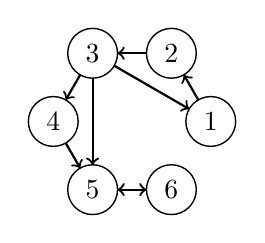
\begin{tikzpicture}
\SetGraphUnit{1}
\Vertices{circle}{1,2,3,4,5,6}
\Edges(1,2,3,1)
\Edges(3,4,5)
\Edges(3,5,6,5)
\end{tikzpicture}
\end{proof}
\begin{thm}[Exercise 1.2.1]
Identify the communicating classes of the following transition matrix:
\begin{gather*}
P=
\begin{pmatrix}\tfrac{1}{2}&0&0&0&\tfrac{1}{2} \\
0&\tfrac{1}{2}&0&\tfrac{1}{2}&0 \\
0&0&1&0&0\\
0&\tfrac{1}{4}&\tfrac{1}{4}&\tfrac{1}{4}&\tfrac{1}{4} \\
\tfrac{1}{2}& 0&0&0&\tfrac{1}{2}\end{pmatrix}
\end{gather*}
\end{thm}

The solution is obvious from the diagram. The classes being \(\{1,5\}, \{2,4\}\) and \(\{3\}\). With  \(\{1,5\}\) closed and \(\{3\}\) absorbing.
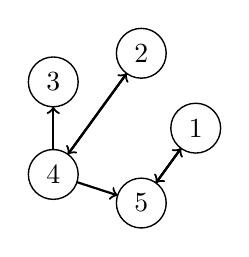
\begin{tikzpicture}
\SetGraphUnit{1}
\Vertices{circle}{1,2,3,4,5}
\Edges(1,5,1)
\Edges(4,2,4,5)
\Edges(4,3)
\end{tikzpicture}

\subsection{Markov Chains 1.3}
\begin{defn}
Let \(X_{n}\) be a Markov chain with transition matrix \(P\). The \emph{hitting time} of a subset \(A\) of \(I\) is the random variable
\[
H^A: \Omega \rightarrow \{0,1,2,\ldots ,\infty \}
\]
given by
\[
H^A(\omega )=\inf\{n\geq 0 :X_{n}(\omega )\in A\}
\]
where we agree that the infimum of the empty set \(\varnothing \) is \(\infty \). The probability starting from \(i\) that \((X_{n})_{n\geq 0}\) ever hits \(A\) is then
\[
h_{i}^A=\Bbb{P}_{i}(H^A<\infty ).
\]
When \(A\) is a closed class, \(h_{i}^A\) is called the \emph{absorption probability}. The mean time taken for \(X_{n}\) to reach \(A\) is given by
\[
k_{i}^A=E_{i}(H^A)=\sum _{n<\infty }n\Bbb{P}(H^A=n)+\infty \Bbb{P}(H^A=\infty ).
\]
We shall often write less formally
\[
h_{i}^A=\Bbb{P}_{i}(\text{hit }A) \qquad k_{i}^A=E_{i}(\text{time to hit }A).
\]
\end{defn}

\begin{thm}[Example 1.3.1]
Consider the chain with following diagram:

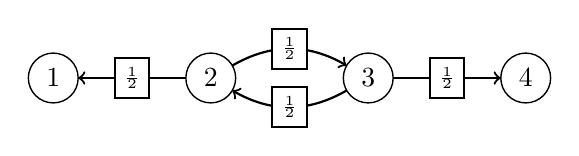
\begin{tikzpicture}
\SetGraphUnit{2}
\Vertices{line}{1,2,3,4}
\Edge[label=\tiny$\tfrac12$](2)(1)
\Edge[label=\tiny$\tfrac12$](3)(4)
\tikzset{EdgeStyle/.append style = {bend left}}
\Edge[label=\tiny$\tfrac12$](2)(3)
\Edge[label=\tiny$\tfrac12$](3)(2)
\end{tikzpicture}

\begin{enumerate}
  \item Starting from 2, what is the probability of absorption in \(4\)?
  \item How long does it take until the chain is absorbed in \(1\) or \(4\) ?
\end{enumerate}
\end{thm}


\begin{proof}
\begin{enumerate}
  \item Note that \(A=\{4\}\) is a closed class. The aborption probability is defined as
\[
h_{i}:=h_{i}^{\{4\}}=\Bbb{P}_{i}(\text{hit } 4).
\]
We have
\begin{align*}
h_{1}&=0 \\
h_{4}&=1 \\
h_{2}&=\tfrac{1}{2}h_{1}+\tfrac{1}{2}h_{3} = \tfrac{1}{2}h_{3} \\
h_{3}&= \tfrac{1}{2}h_{2}+\tfrac{1}{2}h_{4}=\tfrac{1}{2}h_{2}+\tfrac{1}{2}
\end{align*}
Hence
\begin{align*}
&h_{2}=\tfrac{1}{4}h_{2}+\tfrac{1}{4} \\
\Longrightarrow \  &\tfrac{3}{4}h_{2} = \tfrac{1}{4} \\
\Longrightarrow \  &h_{2}=\tfrac{1}{3}
\end{align*}
  \item We need to compute
\[
k_{2}=k_{2}^{\{1,4\}}=E_{2}(\text{time to hit } \{1,4\}).
\]
We have
\begin{gather*}
k_{1}=0 \\
k_{4} = 0 \\
k_{2} = 1+\tfrac{1}{2}k_{3} \\
k_{3} = 1+ \tfrac{1}{2} k_{2}
\end{gather*}
Hence
\begin{align*}
&k_{2} = \tfrac{3}{2} + \tfrac{1}{4} k_{2} \\
\Longrightarrow \ \space &\tfrac{3}{4} k_{2}= \tfrac{3}{2} \\
\Longrightarrow \ \space &k_{2}=2
\end{align*}
\end{enumerate}
\end{proof}

\begin{thm}[Theorem 1.3.2]
The vector of hitting probabilities \(h^A=(h_{i}^A:i\in I)\) is the minimal non-negative solution to the system
\begin{align*}
\begin{cases}h_{i}^A=1 &\text{for}\space i\in A \\ h_{i}^A=\sum _{j\in I}p_{ij}h_{j}^A &\text{for }i\not\in A.\end{cases}
\end{align*}
Minimality means that if \(x=(x_{i}:i\in I)\) is another solution with \(x_{i}\geq 0\) for all \(i\), then \(x_{i}\geq h_{i}\) for all \(i\).
\end{thm}

\begin{thm}[Example 1.3.1(continued)]
Use theorem 1.3.2 to compute \(h_{2}\) again.
\end{thm}

\begin{proof}
The vector of hitting probabilities \(h^{\{4\}}=\Big(h_{1}^{\{4\}},h_{2}^{\{4\}},h_{3}^{\{4\}},h_{4}^{\{4\}}\Big)\) is the minimal non-negative solution to the system
\begin{align*}
&h_{1}^{\{4\}}=\sum _{j\in I}p_{ij}h_{j}^{\{4\}}=h_{1}^{\{4\}}\\
&h_{2}^{\{4\}}=\sum _{j\in I}p_{ij}h_{j}^{\{4\}}=\tfrac{1}{2}h_{1}^{\{4\}}+\tfrac{1}{2}h_{3}^{\{4\}}\\
&h_{3}^{\{4\}}=\sum _{j\in I}p_{ij}h_{j}^{\{4\}}=\tfrac{1}{2}h_{2}^{\{4\}}+\tfrac{1}{2}h_{4}^{\{4\}}\\
&h_{4}^{\{4\}}=1
\end{align*}
The minimality condition gives, that \(h_{1}^{\{4\}}=0\). So that <br />
\begin{align*}
&h_{2}^{\{4\}}=\tfrac{1}{2}h_{3}^{\{4\}}\\
&h_{3}^{\{4\}}=\tfrac{1}{2}h_{2}^{\{4\}}+\tfrac{1}{2}
\end{align*}
which gives:
\begin{align*}
&h_{2}^{\{4\}}=\tfrac{1}{4}h_{2}^{\{4\}}+\tfrac{1}{4}\space \Longrightarrow \space h_{2}^{\{4\}}=\tfrac{1}{3}\\
&h_{3}^{\{4\}}=\tfrac{1}{4}h_{3}^{\{4\}}+\tfrac{1}{2}\space \Longrightarrow \space h_{3}^{\{4\}}=\tfrac{2}{3}
\end{align*}
\end{proof}

\begin{thm}
Consider a recurrence relation of the form
\[
ax_{n+1}+bx_{n}+cx_{n-1}=0 \qquad a,c\neq 0.
\]
Let \(\alpha ,\beta \) be the roots of the quadratic equation
\[
ax^2+bx+c.
\]
Then the general soltuions is given by
\begin{align*}
x_{n}=\begin{cases}A\alpha ^n+B\beta ^n &\text{if }\alpha \neq \beta \\ (A+nB)\alpha ^n &\text{if }\alpha =\beta \end{cases}
\end{align*}
\end{thm}

\begin{prop}
Give a general solution for the recurrence relation
\begin{align*}
h_{0}&=1 \\
h_{i}&=ph_{i+1} +qh_{i-1}
\end{align*}
\end{prop}

\begin{proof}
Note that we have
$-ph_{i+1}+h_{i}-qh_{i-1}=0$. Consider
\[
-px^2+x-1+p=0
\]

We have the roots \(\alpha =1,\beta =\tfrac{q}{p}\). If \(q\neq p\), this gives
\[
h_{i}=A\alpha ^i+B\beta ^i=A+B\Big(\frac{q}{p}\Big)^i.
\]
And if \(p=q\), then \(\alpha =\beta =1,\) and we have
\[
h_{i}=A\alpha ^i+B\beta ^i=A+iB
\]
\(\)
\end{proof}




\begin{thm}[Example 1.3.3]
Consider the Markov chain with diagram

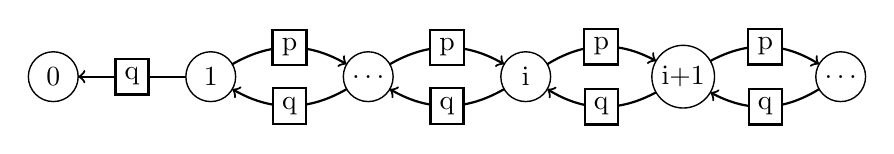
\begin{tikzpicture}
\SetGraphUnit{2}
\Vertices{line}{0,1}
\Vertex[Math,L=\ldots,x=4,y=0] {dots}
\Vertices[x=6,y=0]{line}{i,i+1}
\Vertex[Math,L=\ldots,x=10,y=0] {dots2}
\Edge[label=q](1)(0)
\tikzset{EdgeStyle/.append style = {bend left}}
\Edge[label=p](1)(dots)
\Edge[label=q](dots)(1)
\Edge[label=p](dots)(i)
\Edge[label=q](i)(dots)
\Edge[label=p](i)(i+1)
\Edge[label=q](i+1)(i)
\Edge[label=p](i+1)(dots2)
\Edge[label=q](dots2)(i+1)
\end{tikzpicture}

where \(0<p=1-q<1\). What is \(h_{i}=\Bbb{P}_{i}(\text{hit } 0)\)?
\end{thm}

\begin{proof}
We know that \(h\) is the minimal non-negative solution to
\begin{align*}
h_{0}&=1 \\
h_{i}&=ph_{i+1} +qh_{i-1}
\end{align*}

We consider some cases: 
\begin{itemize}
  \item Suppose \(p=q\), then we have
\[
h_{i}=A\alpha ^i+B\beta ^i=A+iB
\]
and as $0\leq h_{i}\leq 1$ is a probability, we must have $B=0$. We then have
\[
h_{i}=A,
\]
and as \(h_{0}=1,\) we must have $h_{i}=1$.
  \item Suppose $p\neq q$, we then have
\[
h_{i}=A\alpha ^i+B\beta ^i=A+B\Big(\frac{q}{p}\Big)^i.
\]
If \(\frac{q}{p}>1,\) then we must set $B=0$ again.
  \item Suppose \(\frac{q}{p}<1\). We have that $h_{0}=1$, and therefore \(A+B=1.\) Hence:
\[
h_{i}=(\tfrac{q}{p})^i+A\Big(1-(\tfrac{q}{p})^i\Big)
\]
So the minimal non-negative solutions is \(h_{i}=(q/p)^i\).
\end{itemize}
\end{proof}



\begin{thm}[Example 1.3.4]
Consider the Markov chain with diagram

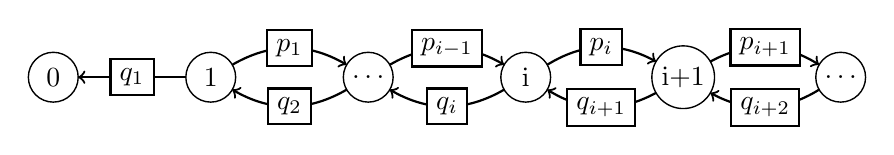
\begin{tikzpicture}
\SetGraphUnit{2}
\Vertices{line}{0,1}
\Vertex[Math,L=\ldots,x=4,y=0] {dots}
\Vertices[x=6,y=0]{line}{i,i+1}
\Vertex[Math,L=\ldots,x=10,y=0] {dots2}
\Edge[label=$q_1$](1)(0)
\tikzset{EdgeStyle/.append style = {bend left}}
\Edge[label=$p_1$](1)(dots)
\Edge[label=$q_2$](dots)(1)
\Edge[label=$p_{i-1}$](dots)(i)
\Edge[label=$q_i$](i)(dots)
\Edge[label=$p_i$](i)(i+1)
\Edge[label=$q_{i+1}$](i+1)(i)
\Edge[label=$p_{i+1}$](i+1)(dots2)
\Edge[label=$q_{i+2}$](dots2)(i+1)
\end{tikzpicture}

where for \(i=1,2,\ldots ,\) we have $0<p_{i}=1-q_{i}<1$. As in the preceding example, $0$ is the absorbing state, and we wish to calculate the absorption probability starting form $i$.
\end{thm}

\begin{proof}
Consider the system of equations
\begin{align*}
h_{0}&=1 \\
h_{i}&=p_{i}h_{i+1}+q_{i}h_{i-1} \qquad\text{for }i=1,2,\ldots 
\end{align*}
Consider
\begin{align*}
u_{i}:&=h_{i-1}-h_{i},
\end{align*}
then
\begin{align*}
&p_{i}u_{i+1}=p_{i}h_{i}-p_{i}h_{i+1}\\
&q_{i}u_{i}=q_{i}h_{i-1}-q_{i}h_{i} \\ \\
\Longrightarrow \  &q_{i}u_{i}-p_{i}u_{i+1}=h_{i}-q_{i}h_{i}-p_{i}h_{i}=0
\end{align*}
Therefore \(p_{i}u_{i+1}=q_{i}u_{i}\) and we have
\[
u_{i+1}=\Big(\frac{q_{i}}{p_{i}}\Big)u_{i}=\prod _{j=1}^i \frac{q_{i}}{p_{i}}u_{1}=\gamma _{1}u_{1}
\]
We also have
\[
u_{1}+\ldots +u_{i}=h_{0}-h_{i}
\]
so
\[
h_{i}=h_{0}-(u_{1}+\ldots +u_{i})=1-u_{1}(\gamma _{0}+\ldots +y_{n-1}).
\]
At this point \(A\) remains to be determined. In the case that \(\sum _{i=0}^\infty \gamma _{i}=\infty \), we must have \(A=0.\) In the other case, we can't take \(A<0,\) but we can take $A>0$ so long as
\[
h_{i}=1-A\sum _{i=0}^{i-1}\gamma _{i} \geq 0.
\]
Which means that
\[
A\leq (\sum _{i=0}^{i-1}\gamma _{i})^{-1}
\]
but still as big as possible. So we get
\[
A=(\sum _{i=0}^{\infty }\gamma _{i})^{-1}.
\]
And therefore
\[
h_{i}=\frac{\sum _{j=i}^{\infty }\gamma _{j}}{\sum _{j=0}^{\infty }\gamma _{j} }
\]
\end{proof}

\begin{thm}[Theorem 1.3.5]
The vector of mean hitting times \(k^A=(k^A:i\in I)\) is the minimal non-negative solution to the system of linear equations
\begin{align*}
\begin{cases}k_{i}^A=0 &\text{for }i\in A \\ k_{i}^A=1+\sum _{j\not\in A}p_{ij}k_{j}^A &\text{for }\not\in A\end{cases}
\end{align*}
\end{thm}


\section{14-10-2014}
\subsection{Markov Chains 1.4}
\begin{defn}
A random variable \(T:\Omega \rightarrow \{0,1,2,\ldots ,\infty \}\) is called a \emph{stopping time} if the event \(\{T=n\}\) depends only on \(X_{0},X_{1},\ldots X_{n}\) for \(n=0,1,2,\ldots \). Intuitively, by watching the process, you know at the time when \(T\) occurs. If asked to stop at \(T\), you know when to stop.
\end{defn}

\begin{prop}
The first passage time
\[
T_{j}=\inf\{n\geq 1:X_{n}=j\}
\]
is a stopping time.
\end{prop}

\begin{proof}
To show that \(T_{j}\) is a stopping time, we have to show that
\[
\{T_{j}=n\}
\]
depends only on \(X_{0},\ldots ,X_{n}\).

This follows from
\[
\{T_{j}=n\}=\{X_{1}\neq j,\ldots X_{n-1}\neq j,X_{n}=j\}
\]
\end{proof}

\begin{prop}
The first hitting time
\[
H^A=\inf\{n\geq 0:X_{n}\in A\}
\]
is a stopping time.
\end{prop}

\begin{proof}
To show that \(H^A\) is a stopping time, we have to show that
\[
\{H^A=n\}
\]
depends only on \(X_{0},\ldots ,X_{n}\).
This follows from
\[
\{H^A=n\}=\{X_{0}\not\in A,\ldots ,X_{n-1}\not\in A,X_{n}\in A\}
\]
\end{proof}

\begin{prop}
The last exit time
\[
L^A=\sup\{n\geq 0:X_{n}\in A\}
\]
is not in general a stopping time.
\end{prop}

\begin{proof}
The event \(\{L^A=n\}\) depends on whether \((X_{n+m})_{m\geq 0}\) visits \(A\) or not. So we don't have a stopping time.
\end{proof}

\begin{thm}[Theorem 1.4.2 (Strong Markov property)]
Let \((X_{n})_{n\geq 0}\) be Markov\((\lambda ,P)\) and let \(T\) be a stopping time of \((X_{n})_{n\geq 0}\). Then, conditional on \(T<\infty \) and \(X_T=i,(X_{T+n})_{n\geq 0}\) is Markov\((\delta _{i},P)\) and independent of \(X_{0},\ldots ,X_T\).
\end{thm}

We now consider an application of the strong Markov property to a Makrov chain \((X_{n})_{n\geq 0}\) observed only at certain times. In the first instance suppose that \(J\) is some subset of the state space \(I\) and that we observe the chain only when it takes values in \(J\).

\begin{prop}
Let \((X_{n})_{n\geq 0}\) be a markov chain. Consider
\[
T_{0}=\inf\{n\geq 0:X_{n}\in J\}
\]
and, for \(m=0,1,2,\ldots \)
\[
T_{m+1}=\inf\{n>T_{m}:X_{n}\in J\}.
\]
Assume \(P(T_{m}<\infty )=1\) for all \(m\). Show that \(Y_{m}=X_{T_{m}}\) is a markov chain and compute its transition matrix in terms of the transition matrix $P$ of $X_{n}$.
\end{prop}
\newpage
\begin{proof}
Showing that \((Y_{m})\) is a markov chain is equivalent with showing that
\begin{align*}
\Bbb{P}(&Y_{m+1}=i_{m+1} | Y_{0}=i_{1},\ldots ,Y_{m}=i_{m} ) \\
&=\Bbb{P}(Y_{m+1}=i_{m+1} | Y_{m}=i_{m})
\end{align*}
which in turn is equivalent with showing that
\begin{align*}
\Bbb{P}(&X_{T_{m+1}}=i_{m+1} | X_{T_{0}} =i_{1},\ldots ,X_{T_{m}}=i_{m} ) \\
&=\Bbb{P}(X_{T_{m+1}}=i_{m+1} | X_{T_{m}}=i_{m} ).
\end{align*}
The Markov property gives that \((X_{T_{m}+n})_{n\geq 0}\) is a markov chain and independent of $X_{0},\ldots ,X_{T_{m}}$, and so surely independent of \(X_{T_{0}} =i_{1},\ldots ,X_{T_{m-1}}\). Now \(X_{T_{m+1}}=X_{T_{m}+n}\) for some $n$. So the equality follows.

Now the question is, strating from $i\in J$ what is the chance that we hit \(j\in J\) the first time we hit \(J\)? Call this chance \(h_{i}^j\) Well this is chance is surely greater than \(p_{ij}\) as there is also a chance that we first get outside of \(J\) and then next time hit \(J\), and so on. With a similar reasoning as in Theorem 1.3.2 we can show that for \(j\in J\) the vector \((h_{i}^j : i\in I)\) is the minimal non-negative solution to
\[
h_{i}^j=p_{ij}+\sum _{k\not\in J}p_{ik}h_{k}^j.
\]

\end{proof}

\begin{prop}
Let \((X_{n})_{n\geq 0}\) be a markov chain. Consider
\[
T_{0}=\inf\{n\geq 0:X_{n}\neq X_{0}\}
\]
and, for \(m=0,1,2,\ldots \)
\[
T_{m+1}=\inf\{n\geq T_{m}:X_{n}\neq X_{T_{m}}\}.
\]
Assume \(\Bbb{P}(T_{m}<\infty )=1\) for all \(m\). Show that \(Y_{m}=X_{T_{m}}\) is a markov chain and compute its transition matrix in terms of the transition matrix $P$ of $X_{n}$.
\end{prop}

\begin{proof}
Showing that \((Y_{m})\) is a markov chain is equivalent with showing that
\begin{align*}
\Bbb{P}(&Y_{m+1}=i_{m+1} | Y_{0}=i_{1},\ldots ,Y_{m}=i_{m} ) \\
&=\Bbb{P}(Y_{m+1}=i_{m+1} | Y_{m}=i_{m})
\end{align*}
which in turn is equivalent with showing that
\begin{align*}
\Bbb{P}(&X_{T_{m+1}}=i_{m+1} | X_{T_{0}} =i_{1},\ldots ,X_{T_{m}}=i_{m} ) \\
&=\Bbb{P}(X_{T_{m+1}}=i_{m+1} | X_{T_{m}}=i_{m} ).
\end{align*}
The Markov property gives that \((X_{T_{m}+n})_{n\geq 0}\) is a markov chain and independent of $X_{0},\ldots ,X_{T_{m}}$, and so surely independent of \(X_{T_{0}} =i_{1},\ldots ,X_{T_{m-1}}\). Now \(X_{T_{m+1}}=X_{T_{m}+n}\) for some $n$. So the equality follows.

Now, the question is, starting from \(i\) what is the chance to go to \(j\) now, if we set the chance \(p_{ii}=0\). Call this chance \(\tilde{p}_{ij}\). We have
\[
\tilde{p}_{ij}=\frac{p_{ij}}{\sum \limits_{k\neq i}p_{ik}}
\]
\end{proof}
\subsection{Markov Chains 1.5}
\begin{defn}
Let \((X_{n})_{n\geq 0}\) be a Markov chain with transition matrix \(P\). We say that a state \(i\) is \emph{recurrent} if
\[
\Bbb{P}_{i}(X_{n}=i \text{ for infinitely many }n)=1.
\]
A recurrent state is a state \(i\) where you keep coming back.
\end{defn}

\begin{defn}
We say that a state \(i\) is \emph{transient} if
\[
\Bbb{P}_{i}(X_{n}=i \text{ for infinitely many }n)=0.
\]
A transient state is a state \(i\) which you eventually leave for ever.
\end{defn}

\begin{thm}
A state \(i\) is either recurrent or transient.
\end{thm}

\begin{defn}
Recall that the first passage time to a state \(i\) is the random variable \(T_{i}\) defined by
\[
T_{i}(\omega )=\inf\{n\geq 1 : X_{n}(\omega )=i\}
\]
where \(\inf \varnothing =\infty .\) We now define inductively the \emph{rth passage time} \(T_{i}^{(r)}\) to state \(i\) by
\[
T_{i}^{(0)}(\omega )=0 \quad T_{i}^{(1)}(\omega )=T_{i}(\omega )
\]
and for \(r=0,1,2,\ldots ,\)
\[
T_{i}^{(r+1)}(\omega )=\inf\{n\geq T_{i}^{(r)}(\omega )+1 : X_{n}(\omega )=i\}.
\]
The length of the rth excursion to \(i\) is then
\begin{align*}
S_{i}^{(r)}=\begin{cases}T_{i}^{(r)}-T_{i}^{(r-1)} &\text{if }T_{i}^{(r-1)}<\infty  \\0 & \text{otherwise}\end{cases}.
\end{align*}
\end{defn}

\begin{thm}[Lemma 1.5.1]
For \(r=2,3,\ldots ,\) conditional on \(T_{i}^{(r-1)}<\infty \), \(S_{i}^{(r)}\) is independent of
\(\{X_{m}:m\leq T_{i}^{(r-1)}\}\) and
\[
\Bbb{P}(S_{i}^{(r)}=n|T_{i}^{(r-1)}<\infty )=\Bbb{P}_{i}(T_{i}=n)
\]
\end{thm}

\begin{defn}
The \emph{number of visits} to \(i\) is denoted by
\[
V_{i}=\sum _{n=0}^\infty 1_{\{X_{n}=i\}}.
\]

\end{defn}

\begin{thm}
\[
E_{i}(V_{i})=\sum _{n=0}^\infty p_{ii}^{(n)}
\]
\end{thm}

\begin{proof}
We have
\begin{align*}
E_{i}(V_{i}) &=\sum _{n=0}^\infty E_{i}(1_{\{X_{n}=i\}}) \\
&=\sum _{n=0}^\infty  \Bbb{P}_{i}(X_{n}=i) \\
&=\sum _{n=0}^\infty p_{ii}^{(n)} 
\end{align*}
\end{proof}

\begin{defn}
The \emph{return probability} of \(i\) is denoted by
\[
f_{i}=\Bbb{P}_{i}(T_{i}<\infty ).
\]
\end{defn}

\begin{thm}[Lemma 1.5.2]
For \(r=0,1,2,\ldots ,\) we have \(\Bbb{P}_{i}(V_{i}>r)=f_{i}^r.\)
\end{thm}

\begin{proof}
Showing that
\[
\Bbb{P}_{i}(V_{i}>r)=f_{i}^r
\]
is equivalent with showing that
\[
\Bbb{P}_{i}(V_{i}>r)=\Bbb{P}_{i}(T_{i}<\infty )^r
\]
which in turn is equivalent with
\[
\Bbb{P}_{i}(T_{i}^{(r)}<\infty )=\Bbb{P}_{i}(T_{i}<\infty )^r.
\]
This last statement can be proven by induction.
\end{proof}

\begin{thm}[Theorem 1.5.3]
The following dichotomy holds:

\begin{enumerate}
  \item if \(\Bbb{P}_{i}(T_{i}<\infty )=1,\) then \(i\) is recurrent and \(\sum _{n=0}^\infty p_{ii}^{(n)}=\infty \)
  \item if \(\Bbb{P}_{i}(T_{i}<\infty )<1,\) then \(i\) is transient and \(\sum _{n=0}^\infty  p_{ii}^{(n)}<\infty \)
\end{enumerate}
\end{thm}


\begin{thm}[Theorem 1.5.4]
Let \(C\) be a communicating class. Then either all states in \(C\) are transient or all are recurrent.
\end{thm}

\begin{thm}[Theorem 1.5.5]
Every recurrent class is closed. And the contrapositive: \\
Every class that is not closed, is transient. 
\end{thm}

\begin{thm}[Theorem 1.5.6]
Every finite closed class is recurrent.
And the contrapositive: \\
Every transient class is either infinite or not closed.. 
\end{thm}

\begin{thm}[Theorem 1.5.7]
Suppose \(P\) is irreducible and recurrent. Then for all \(j\in I\) we have
\[
\Bbb{P}(T_{j}<\infty )=1.
\]
\end{thm}


\begin{thm}[Exercise 1.5.1]
Identify the recurrent and transient states of the Markov chain with the following transition matrix:
\begin{gather*}
P=
\begin{pmatrix}\tfrac{1}{2}&0&0&0&\tfrac{1}{2} \\
0&\tfrac{1}{2}&0&\tfrac{1}{2}&0 \\
0&0&1&0&0\\
0&\tfrac{1}{4}&\tfrac{1}{4}&\tfrac{1}{4}&\tfrac{1}{4} \\
\tfrac{1}{2}& 0&0&0&\tfrac{1}{2}\end{pmatrix}
\end{gather*}
\end{thm}

The solution is obvious from the diagram:

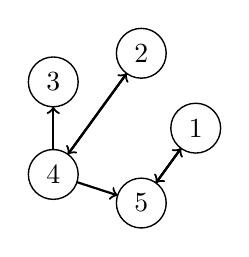
\begin{tikzpicture}
\SetGraphUnit{1}
\Vertices{circle}{1,2,3,4,5}
\Edges(1,5,1)
\Edges(4,2,4,5)
\Edges(4,3)
\end{tikzpicture}

 The classes being \(\{1,5\}, \{2,4\}\) and \(\{3\}\). With  \(\{1,5\}\) closed and finite, and therefore recurrent. The class \(\{3\}\) is absorbing, so closed and finite, and therefore recurrent. The other class $\{2,4\}$ is not closed, and therefore, not recurrent. So we have that $\{2,4\}$ is transient.



\section{15-10-2014}
\subsection{Markov Chains 1.6}

\begin{thm}
A state \(i\) is recurrent if and only if \(\sum _{n=0}^\infty p_{ii}^{(n)}=\infty .\)
\end{thm}

\begin{thm}[Example 1.6.1 The simple random walk on \(\Bbb{Z}\)]
Compute \(\sum _{n=0}^\infty p_{00}^{(n)}.\)
\end{thm}

\begin{proof}
First note that \(p_{00}^{(2n+1)}=0.\)

Any given sequence of steps of length \(2n\) from \(0\) to \(0\) occurs with probability \(p^nq^n\), there being \(n\) steps up and \(n\) steps down. And the number of such sequences is the number of ways of choosing the \(n\) steps up from \(2n\). Thus
\[
p_{00}^{(2n)}={2n\choose n}p^nq^n=\frac{(2n)!}{n!^2}(pq)^n.
\]
Remember that
\[
n! \simeq  \sqrt {2\pi n}(n/e)^n  \qquad n\rightarrow \infty .
\]
So
\begin{align*}
(2n)! &\simeq  \sqrt {4\pi n}(2n/e)^{2n}  &\qquad n\rightarrow \infty \\
n!^{2} &\simeq  {2\pi n}(n/e)^{2n}  &\qquad n\rightarrow \infty .
\end{align*}
And therefore
\begin{align*}
\frac{(2n)!}{n!^2}(pq)^n\simeq \frac{(4pq)^n}{\sqrt {\pi n}} &\qquad n\rightarrow \infty 
\end{align*}

\begin{itemize}
  \item \(p=q:\) Then \(p=q=1/2\), so \(4pq=1\). And we have
\begin{align*}
p_{00}^{(2n)}\simeq \frac{1}{\sqrt {\pi n}} &\qquad n\rightarrow \infty 
\end{align*}
which is equivalent with
\[
\forall \epsilon>0\  \exists N:n\geq N\Longrightarrow \frac{1}{\sqrt {\pi }\sqrt {n}}-\epsilon<p_{00}^{(2n)}<\frac{1}{\sqrt {\pi n}}+\epsilon.
\]
So there exists a \(N\) such that for all \(n\geq N\) we have
\[
p_{00}^{(2n)}>\frac{1}{2\sqrt n}.
\]
Therefore
\[
\sum _{n=0}^\infty p_{00}^{(n)}>\sum _{n=N}^\infty p_{00}^{(2n)}>\sum _{n=N}^\infty \frac{1}{2\sqrt n}=\infty 
\]
  \item \(p\neq q:\) Then \(4pq=r<1.\) And we have
\begin{align*}
p_{00}^{(2n)}\simeq \frac{r^n}{\sqrt {\pi n}} &\qquad n\rightarrow \infty 
\end{align*}
which is equivalent with
\[
\forall \epsilon>0\  \exists N:n\geq N\Longrightarrow \frac{r^n}{\sqrt {\pi }\sqrt {n}}-\epsilon<p_{00}^{(2n)}<\frac{r^n}{\sqrt {\pi n}}+\epsilon.
\]
So there exists a \(N\) such that for all \(n\geq N\)  we have
\[
p_{00}^{(2n)}<r^n
\]
Therefore
\[
\sum _{n=N}^\infty p_{00}^{(n)}=\sum _{n=N}^\infty p_{00}^{(2n)}<\sum _{n=N}^\infty r^n<\infty .
\]
And therefore
\[
\sum _{n=0}^\infty p_{00}^{(n)}<\infty .
\]
\end{itemize}

\end{proof}

\begin{thm}[Example 1.6.2 The simple random walk on \(\Bbb{Z}^{2}\)]
Compute \(\sum _{n=0}^\infty p_{00}^{(n)}.\)
\end{thm}

\begin{proof}
By rotating \(\Bbb{Z}^{2}\) we get that each step is like moving in one step in each of the independent, one dimensional, simple random walks. Hence
\[
p_{00}^{(2n)}\simeq \bigg(\frac{1}{\sqrt {\pi n}}\bigg)^2=\frac{1}{\pi n}
\]
which is equivalent with
\[
\forall \epsilon>0\  \exists N:n\geq N\Longrightarrow \frac{1}{\pi n}-\epsilon<p_{00}^{(2n)}<\frac{1}{\pi n}+\epsilon.
\]
So there exists a \(N\) such that for all \(n\geq N\) we have
\[
p_{00}^{(2n)}>\frac{1}{4n}.
\]
Therefore
\[
\sum _{n=0}^\infty p_{00}^{(n)}>\sum _{n=N}^\infty p_{00}^{(2n)}>\frac{1}{4}\sum _{n=N}^\infty \frac{1}{n}=\infty 
\]

\end{proof}
\subsection{Markov Chains 1.7}
\begin{defn}
We say that a measure \(\lambda =(\lambda _{i}: i\in I)\) where \(\lambda _{i}\geq 0\) is \emph{invariant} if
\[
\lambda P=\lambda .
\]
\end{defn}

\begin{thm}[Theorem 1.7.1]
Let \((X_{n})_{n\geq 0}\) be a Markov\((\lambda ,P)\) and suppose that \(\lambda \) is invariant for \(P\). Then \((X_{n+m})_{n\geq 0}\) is also Markov \((\lambda ,P)\).
\end{thm}

\begin{thm}[Theorem 1.7.2]
Let \(I\) be finite. Suppose for some \(i\in I\) that for all \(j\in J\)
\[
p_{ij}^{(n)}\rightarrow \pi _{j} \qquad n\rightarrow \infty .
\]
Then \(\pi =(\pi _{j}:j\in I)\) is an invariant distribution.
\end{thm}

\begin{prop}
Give a example of infinite state space \(I\) where Theorem 1.7.2 doesn't hold.
\end{prop}

\begin{proof}
For the random walk in \(\Bbb{Z}\) we have for all \(i,j\in I\)
\[
p_{ij}^n\rightarrow 0 \qquad n\rightarrow \infty .
\]
Note however that \((0,0,\ldots )\) is not a distrubution. As the total mass
\[
\sum _{i\in I}\lambda _{i}=0\neq 1.
\]
\end{proof}


\begin{thm}
Consider a recurrence relation of the form
\[
x_{n+1}=ax_{n}+b.
\]
The general solution is
\[
x_{n}=\begin{cases}Aa^n+b/(1-a) &a\neq 1\\ x_{n}=x_{0}+nb &a=1\end{cases}
\]
\end{thm}

\begin{thm}[Example 1.1.4]
The most general two-state chain has transition matrix of the form
\[
P= \begin{pmatrix}1-\alpha &\alpha  \\ \beta &1-\beta \end{pmatrix}.
\]
Draw the diagram, and find \(p_{11}^{(n)}.\)
\end{thm}

\begin{proof}
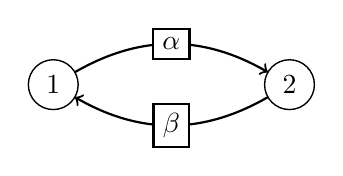
\begin{tikzpicture}
\SetGraphUnit{3}
\Vertices{line}{1,2}
\tikzset{EdgeStyle/.append style = {bend left}}
\Edge[label=$\beta$](2)(1)
\Edge[label=$\alpha$](1)(2)
\end{tikzpicture}

We have that
\[
P^{n+1}=P^n\begin{pmatrix}1-\alpha &\alpha  \\ \beta &1-\beta \end{pmatrix}.
\]
And therefore
\[
p_{11}^{(n+1)}=p_{11}^{(n)}(1-\alpha )+ p_{12}^{(n)}\beta .
\]
Note that we have
\[
p_{12}^{(n)}=1-p_{11}^{(n)}.
\]
So we have
\[
p_{11}^{(n+1)}=p_{11}^{(n)}(1-\alpha -\beta )+ \beta .
\]
The general solution of this recurrence relation is
\[
p_{11}^{(n)}=
\begin{cases}A(1-\alpha +\beta )^n+\alpha /(\alpha +\beta ) &(1-\alpha +\beta )\neq 1 \\
1+n\beta  &1-\alpha +\beta =1\end{cases}
\]

This reduces to:
\[
p_{11}^{(n)}=
\begin{cases}\frac{\beta }{\alpha +\beta } (1-\alpha +\beta )^n+\alpha /(\alpha +\beta ) &\alpha +\beta >0 \\
1 &\alpha =\beta =0\end{cases}
\]

\end{proof}


\begin{prop}
Consider the two-state Markov chain with transition matrix
\[
P=
\begin{pmatrix}1-\alpha &\alpha \\
\beta &1-\beta \end{pmatrix}
\]
Ignore the trivial cases \(\alpha =\beta =0\) and \(\alpha =\beta =1.\)
\end{prop}

\begin{proof}
From example 1.1.4 we have
\[
p_{11}^{(n)}=
\begin{cases}\frac{\alpha }{\alpha +\beta } (1-\alpha -\beta )^n+\beta /(\alpha +\beta ) &\alpha +\beta >0 \\
1 &\alpha =\beta =0\end{cases}
\]
In a similar we could have shown that
\[
p_{12}^{(n)}=
\begin{cases}\frac{\alpha }{\alpha +\beta } (1-\alpha -\beta )^n+\alpha /(\alpha +\beta ) &\alpha +\beta >0 \\
1 &\alpha =\beta =0\end{cases}
\]

Therefore \(p_{11}^{(n)}\rightarrow \frac{\beta }{\alpha +\beta }\) and \(p_{12}^{(n)}\rightarrow \frac{\alpha }{\alpha +\beta }\). And by theorem 1.7.2 we get that
\[
\bigg(\frac{\beta }{\alpha +\beta },\frac{\alpha }{\alpha +\beta }\bigg)
\]
is an invariant distribution.
\end{proof}

\begin{defn}
For a fixed state \(k\), consider for each \(i\) the expected time spent in \(i\) between visits to \(k\):
\[
\gamma _{i}^k=E_{k} \sum _{n=0}^{T_{k}-1}1_{\{X_{n}=i\}}
\]
\end{defn}

\begin{thm}[Theorem 1.7.5]
Let \(P\) be irreducible and recurrent. Then

\begin{enumerate}
  \item \(\gamma _{k}^k=1\)
  \item \(\gamma ^k=(\gamma _{i}^k:i\in I)\) satisfies \(\gamma ^kP=\gamma ^k\)
  \item \(0<\gamma _{i}^k<\infty \) for all \(i\in I\)
\end{enumerate}
\end{thm}


\begin{thm}[Theorem 1.7.6]
Let \(P\) be irreducible and let \(\lambda \) be an invariant measure for \(P\) with \(\lambda _{k}=1\). Then \(\lambda \geq \gamma ^k\). If in addition \(P\) is recurrent, then \(\lambda =\gamma ^k\).
\end{thm}

Recall that a state \(i\) is recurrent if
\[
\Bbb{P}_{i}(X_{n}=i \text{ for infinitely many } n)=1
\]
and we showed in Theorem 1.5.3 that this is equivalent to
\[
\Bbb{P}_{i}(T_{i}<\infty )=1.
\]

\begin{defn}
We call a recurrent state \(i\) positive recurrent if
\[
m_{i}=E_{i}(T_{i})<\infty .
\]
If a recurrent state fails to have this stronger property we call it \emph{null recurrent}.
\end{defn}

\begin{thm}[Theorem 1.7.7]
Let \(P\) be irreducible. Then the following are equivalent:

\begin{enumerate}
  \item every state is positive recurrent
  \item some state \(i\) is positive recurrent
  \item \(P\) has an invariant distribution \(\pi \)
\end{enumerate}

\end{thm}

\begin{thm}
If \(P\) has an invariant distribution \(\pi \), we have that \(m_{i}=E_{i}(T_{i})=\frac{1}{\pi _{i}}\) for all \(i\).
\end{thm}

\begin{thm}[Example 1.7.8]
Show that the simple symmetric random walk on \(\Bbb{Z}\) is null recurrent.
\end{thm}

\begin{proof}
The simple symmetric random walk on \(\Bbb{Z}\) is irreducible and, by example 1.6.1, it also recurrent.  Remember that
\[
(\pi P)_{j}=\sum _{i\in I}\pi _{i}p_{ij}
\]
and this equals to
\[
\sum _{i\in I}\pi _{i}p_{ij}=1/2 \pi _{j-1}+1/2\pi _{j+1}.
\]
So
\[
\pi _{i}=\tfrac{1}{2}\pi _{i-1}+\tfrac{1}{2}\pi _{i+1}.
\]
We get the equation
\[
x^2-2x+1=0.
\]
And so we have
\[
\alpha =\beta =1.
\]
And so the general solutions is
\[
\pi _{i}=A+iB.
\]
and the total mass is then
\[
\sum _{i}\pi _{i}=A\sum _{i}1+B\sum _{i}i=B\infty .
\]
So whatever \(A,B\) we choose, we never get the total mass to be zero. So there doesn't exists a invariant distribution, and by Theorem 1.7.7 we have that all states must be null recurrent.
\end{proof}
\newpage
\begin{thm}[Example 1.7.9]
Show that the existence of an invariant measure does not guarantee recurrence.
\end{thm}

\begin{proof}
The simple symmetric random walk on \(\Bbb{Z}^{3}\) has an invariant measure. Consider:
\[
(\pi P)_{j}=\sum _{i\in I}\pi _{i}p_{ij}=1/4(\pi _{a}+\pi _{b}+\pi _{c}+\pi _{d})
\]
So if we set \(\pi =(1,1,1,\ldots )\). Then \(\pi \) is invariant. But \(\Bbb{Z}^{3}\) is also transient.
\end{proof}

\begin{thm}[Example 1.7.10]
Consider the asymmetric random walk on \(\Bbb{Z}\) with transition probabilities
\(p_{i,i-1}=q<p=p_{i,i+1}\). Show that the walk is null recurrent.
\end{thm}

\begin{proof}
We have
\begin{align*}
\pi _{j}=(\pi P)_{j}&=\sum _{i\in I}\pi _{i}p_{ij}=\pi _{j-1}p_{j-1,j}+\pi _{j+1}p_{j+1,j} \\
&=\pi _{j-1}p+\pi _{j+1}q
\end{align*}
This is a recurrence relation and we have the equation
\begin{gather*}
qx^2-x+p=0  \\
D=\sqrt {1-4(1-p)p}=\sqrt {1-4p+4p^2}=1-2p \\
\alpha =\frac{-1+1-2p}{-2p}=1 \qquad \beta =\frac{-2+2p}{-2p}=\frac{1-p}{p}=\frac{q}{p}
\end{gather*}
So we have the general solution:
\[
\pi _{j}=A\alpha ^j+B\beta ^j=A+B\Big(\frac{p}{q}\Big)^i.
\]
And the total mass is therefore
\[
\sum _{j=0}^\infty \pi _{j}=\sum _{j=0}^\infty A+B\Big(\frac{p}{q}\Big)^i=B\infty .
\]

So whatever \(A,B\) we choose, we never get the total mass to be zero. So there doesn't exists a invariant distribution, and by Theorem 1.7.7 we have that all states must be null recurrent.

\end{proof}

\begin{thm}[Example 1.7.11]
Consider a success-run chain on \(\Bbb{Z}^+\), whose transition probabilities given by
\[
p_{i,i+1}=p_{i} \qquad p_{i0}=q_{i}=1-p_{i}.
\]
And where
\[
p=\prod _{i=0}^\infty p_{i}>0.
\]
Show that every state is transient.
\end{thm}

\begin{proof}
We have
\begin{align*}
\pi _{j}=(\pi P)_{j}&=\sum _{i\in I}\pi _{i}p_{ij} \\
&=\pi _{j-1}p_{j-1}\\
&=\pi _{0}\prod _{i=0}^{j-1}p_{i}
\end{align*}
and
\begin{align*}
\pi _{0}&=\sum _{i=0}^\infty \pi _{i}p_{i0}\\
&=\sum _{i=0}^\infty (1-p_{i})\pi _{i} \\
&=\pi _{0}\sum _{i=0}^\infty (1-p_{i})\prod _{j=0}^{i-1}p_{j} \\
&=\pi _{0}\sum _{i=0}^\infty \prod _{j=0}^{i-1}p_{j}-\prod _{j=0}^{i}p_{j} \\
&=\pi _{0}(1-\prod _{j=0}^{\infty }p_{j}).
\end{align*}
The last equality need some thinking, but notice that it's a telescoping sum. Define

$$a_i := \prod_{j=0}^{i-1} p_j,$$

the sum is

$$\sum_{i=0}^\infty (a_i - a_{i+1}) = a_0 - \lim_{k\to\infty} a_k= 1-\prod _{j=0}^{\infty }p_{j}$$

The equation 
\[\pi _{0}=\pi _{0}(1-\prod _{j=0}^{\infty }p_{j})\]
forces \(\pi _{0}\) to be \(0\). And therefore all \(\pi _{i}\) are zero. So there is no invariant distribution and we have that \(P\) is transient by theorem 1.7.7.
\end{proof}




%Week 2
\section{16-10-2014}
\subsection{Markov Chains 1.8}

\begin{prop}
Give an example where the limit \(p_{ij}^{(n)}\) fails to converge.
\end{prop}
\begin{proof}
Consider the two-state chain with transition matrix
\begin{gather*}
P=\begin{pmatrix}0&1\\ 1&0\end{pmatrix}.
\end{gather*}

Then \begin{gather*}
P^2=\begin{pmatrix}0&1\\ 1&0\end{pmatrix}\begin{pmatrix}0&1\\ 1&0\end{pmatrix}=I.
\end{gather*}
So \(P^2=I\), so \(P^{2n}=I.\) And \(P^{2n+1}=P.\) Thus \(p_{ij}^{(n)}\) fails to converge for all \(i,j\).
\end{proof}

\begin{defn}
We call a state \(i\) \emph{aperiodic} if \(p_{ii}^{(n)}>0\) for all sufficiently large \(n\).
\end{defn}

\begin{thm}
A state \(i\) is aperiodic if and only if the set
\(\{n\geq 0: p_{ii}^{(n)}>0\}\) has no common divisor other than \(1.\)
\end{thm}

\begin{thm}[Lemma 1.8.2]
Suppose \(P\) is irreducible and has an aperiodic state \(i\). Then, for all states \(j\) and \(k\), \(p_{jk}^{(n)}>0\) for all sufficiently large \(n\). In particular, all states are aperiodic.
\end{thm}

\begin{thm}[Theorem 1.8.3]
Let \(P\) be irreducible and aperiodic, and suppose that \(P\) has an invariant distribution \(\pi \). Let \(\lambda \) be any distribution. Suppose that
\((X_{n})_{n\geq 0}\) is Markov\((\lambda ,P)\). Then for all \(j\)
\[
\Bbb{P}(X_{n}=j)\rightarrow \pi _{j} \qquad n\rightarrow \infty .
\]
In particular, for all \(i,j\)
\[
p_{ij}^{(n)}\rightarrow \pi _{j} \qquad n\rightarrow \infty 
\]
\end{thm}

\subsection{Representation Theory Week 39}

Let \(k\) be a field. And let \(A\) be a \(k\)-algebra.

\begin{defn}
An element \(a\in A\) is called an \emph{idempotent element} or an \emph{idempotent} if \(a^2=a.\)
\end{defn}

\begin{prop}
We have that \(0\) and \(1\) are idempotents of \(A\).
\end{prop}

\begin{defn}
Two idempotents \(a,b\in A\) are called \emph{orthogonal} if \(ab=0\) and \(ba=0\).
\end{defn}

\begin{prop}
If \(a,b\) are orthogonal, then \(a+b\) is an idempotent.
\end{prop}

\begin{proof}
Showing that \(a+b\) is idempotent, is equivalent with showing that
\[
(a+b)^2=a+b
\]
which is equivalent with showing that
\[
a+ab+ba+b=a+b
\]
which in turn is equivalent with showing that
\[
ab+ba=0.
\]
It suffices to show that
\[
ab=0=ba.
\]
By hypothesis we have that $a,b$ are orthogonal, and therefore our last statement follows by definition.
\end{proof}

\begin{defn}
A set of mutually orthogonal idempotents \(a_{1},\ldots ,a_{n}\in A\) is called \emph{complete} if
\[
1=a_{1}+\cdots +a_{n}.
\]
\end{defn}

\begin{defn}
An idempotent \(a\in Z(A)\) is called a \emph{central idempotent} of \(A\).
\end{defn}

\begin{defn}
A nonzero idempotent \(a\in A\) is called \emph{minimal} if any decomposition of \(a\) as a sum of two orthogonal idempotents \(a=b+c\) implies that \(b=0\) or \(c=0\).
\end{defn}

\begin{prop}
If \(V\) is a \(k\)-vector space, then \(\End_{k}(V)\) is a \(k\)-algebra.
\end{prop}

\begin{proof}
Showing that \(\End_{k}(V)\) is a \(k\)-algebra is equivalent with showing that there exists a ring homomorphism
\[
f: k \rightarrow  Z(\End_{k}(V))
\]
which is equivalent with showing that there exists a map \(f\) such that

\begin{enumerate}
  \item \(f(\alpha )L=Lf(\alpha ) \qquad \forall \alpha \in k,\forall L\in \End_{k}(V)\)
  \item \(f(\alpha )f(\beta )=f(\alpha \beta ) \qquad \forall \alpha ,\beta \in k\)
  \item \(f(\alpha )+f(\beta )=f(\alpha +\beta ) \qquad \forall \alpha ,\beta \in k\)
\end{enumerate}

Remember that the condition in 1) implies that \(f(\alpha )\) must be a scalar. Let's try the mapping \(f(\alpha )=\alpha I\) and rewrite our conditions:

\begin{enumerate}
  \item \(\alpha I\circ L=L\circ \alpha I \qquad \forall \alpha \in k,\forall L\in \End_{k}(V)\)
  \item \(\alpha I\beta I=(\alpha \beta )I \qquad \forall \alpha ,\beta \in k\)
  \item \((\alpha +\beta )I=\alpha I+\beta I \qquad \forall \alpha ,\beta \in k\)
\end{enumerate}

All those conditions hold directly.
\end{proof}

\begin{prop}
If \(V\) is a representation of a \(k\)-algebra \(A\), then \(\End_A(V)\) is a \(k\)-algebra.
\end{prop}

\begin{proof}
Showing that \(\End_A(V)\) is a \(k\)-algebra is equivalent with showing that there exists a ring homomorphism
\[
f: k \rightarrow  Z(\End_A(V))
\]
which is equivalent with showing that there exists a map \(f\) such that

\begin{enumerate}
  \item \(f(\alpha )L=Lf(\alpha ) \qquad \forall \alpha \in k,\forall L\in \End_A(V)\)
  \item \(f(\alpha )f(\beta )=f(\alpha \beta ) \qquad \forall \alpha ,\beta \in k\)
  \item \(f(\alpha )+f(\beta )=f(\alpha +\beta ) \qquad \forall \alpha ,\beta \in k\)
\end{enumerate}

Remember that the condition in 1) implies that \(f(\alpha )\) must be a scalar. Let's try the mapping \(f(\alpha )=\alpha .I\) and rewrite our conditions:

\begin{enumerate}
  \item \(\alpha .I\circ L=L\circ \alpha .I \qquad \forall \alpha \in k,\forall L\in \End_{k}(V)\)
  \item \(\alpha .I\beta .I=(\alpha \beta ).I \qquad \forall \alpha ,\beta \in k\)
  \item \((\alpha +\beta ).I=\alpha .I+\beta .I \qquad \forall \alpha ,\beta \in k\)
\end{enumerate}

All those conditions hold directly.
\end{proof}

\begin{prop}
\[
\End_A(V)\subseteq \End_{k}(V)
\]
\end{prop}

\begin{proof}
Showing that \(\End_A(V)\subseteq \End_{k}(V)\) is equivalent with showing that
\[
\phi \in \End_A(V) \Longrightarrow  \phi \in  \End_{k}(V).
\]
In other words, does \(A\)-linearity imply \(k\)-linearity ? This holds as \(k1\subseteq A\).
\end{proof}

\begin{prop}
Given a representation \(V\) of \(A\). Then \(V\) is also a representation of \(\End_A(V)\)
\end{prop}

\begin{proof}
To show that \(V\) is a representation of \(\End_A(V)\) it suffices to show that there exists a homomorphism of algebras:
\[
\rho :\End_A(V)\rightarrow \End_{k}(V).
\]
Remember that we have \(\End_A(V)\subseteq \End_{k}(V).\) So we can define \(\rho \) just as the inclusion map, which is clearly a homomorphism of algebras.
\end{proof}

\begin{defn}
Given a representation \(V\) of \(A\). Then \(V\) as representation of \(A':=\End_A(V)\) is called the \emph{centralizer module}. If we need to distinguish the two module structures on \(V\), we will write \(_AV\) to denote \(V\) as a module over \(A\), and \(_{A'}V\) to denote the centralizer module.
\end{defn}

\begin{prop}
The image of an idempotent element under an algebra homomorphism is again an idempotent element.
\end{prop}

\begin{proof}
Let \(a\in A:a^2=a\). It suffices to show that
\[
f(a)^2=f(a).
\]
This holds as:
\[
f(a)^2=f(a)f(a)=f(a^2)=f(a).
\]
\end{proof}

\begin{prop}
For any idempotent \(e\in A\) we have that

\begin{enumerate}
  \item \(\rho (e)\in \End_{k}(V)\) is idempotent
  \item if \(e\) is central, then \(\rho (e)\in \End_A(V)\)
\end{enumerate}
\end{prop}


\begin{proof}

\begin{enumerate}
  \item The statement holds as \(\rho \) is an algebra homomorphism. And remember that the image of an idempotent element under an algebra homomorphism is again an idempotent element.
  \item Showing that
\[
\rho (e)\in \End_A(V)
\]
is equivalent with showing that
\[
a.\rho (e)(v)=\rho (e)(a.v)
\]
which in turn is equivalent with
\[
\rho (a)(\rho (e)(v))=\rho (e)(\rho (a)(v)).
\]
In other notation
\[
\rho (a)\circ \rho (e)(v)=\rho (e)\circ \rho (a)(v).
\]
As \(\rho \) is an algebra homomorphism this is equivalent with
\[
\rho (ae)(v)=\rho (ea)(v).
\]
By hypothesis, we have that \(e\) is central, so \(ea=ae\) and therefore our last statement holds. 
\end{enumerate}
\end{proof}


\begin{prop}
For any \(x\in \End_A(V)\) the subspace \(\Ker(x)\subseteq V\) is a \(A\)-submodule.
\end{prop}

\begin{proof}
Showing that \(\Ker(x)\) is a subrepresentation of \(V\) is equivalent with showing that
\[
a.\Ker(x)\subseteq \Ker(x) \qquad \forall a\in A.
\]
which is equivalent with showing that
\[
x(a.v)=0 \qquad \forall a\in A,\forall v\in \Ker(x)
\]
As \(x\in \End_A(V)\), this is equivalent with showing that
\[
a.x(v)=0 \qquad \forall a\in A,\forall v\in \Ker(x) \qquad \checkmark.
\]
\end{proof}

\begin{prop}
For any \(x\in \End_A(V)\) the subspace \(\I(x)\subseteq V\) is a \(A\)-submodule.
\end{prop}

\begin{proof}
Showing that \(\I(x)\) is a subrepresentation is equivalent with showing that
\[
a.\I(x)\subseteq \I(x)
\]
which is equivalent with showing that
\[
\forall a\in A\  \forall v\in V\  \exists w\in W \qquad a.x(v)=x(w) 
\]
As \(x\in \End_A(V)\), this is equivalent with showing that
\[
\forall a\in A\forall v\in V\  \exists w\in W \qquad x(a.v)=x(w) \qquad \checkmark. 
\]
\end{proof}

\begin{prop}
If \(V=U\oplus W\) is a decomposition of \(_AV\) as direct sum of \(A\)-submodules. Then the projection \(e_U\) of \(V\) onto \(U\) along \(W\) and the projection \(e_W\) of \(V\) onto \(W\) along \(U\) satisfy:

\begin{enumerate}
  \item \(e_U,e_W\in \End_A(V)\)
  \item \(e_U\) and \(e_W\) are orthogonal idempotent elements
  \item \(1=e_U+e_W\)
\end{enumerate}

\end{prop}

Remember that if \(V=U\oplus W\), then we can regard $U,W$ as subspaces of \(V\) such that \(U\cap W=0\) and for any \(v\in V\) we have that \(v=u+w\) where \(u\in U, w\in W\). And \(a.v=a.u+a.w\) where \(a.u\in U\)

\begin{proof}[Proof of 1]
To show that \(e_U\in \End_A(V)\) it suffices to show that
\[
a.e_U(v)= e_U(a.v) \qquad \forall a\in A,v\in V
\]
which is equivalent with showing that
\[
a.e_U(u+w)= e_U(a.(u+w)) \qquad \forall a\in A,u\in U,w\in W
\]
which is equivalent with showing that
\[
a.u= e_U(a.u+a.w) \qquad \forall a\in A,u\in U,w\in W.
\]
With holds as \(U,W\) are subrepresentations.
\end{proof}

\begin{proof}[Proof of 2]
Showing that \(e_U\) is idempotent, is equivalent with showing that
\[
e_U\circ e_U=e_U
\]
which is equivalent with showing that
\[
e_U\circ e_U(v)=e_U(v) \qquad \forall v\in V
\]
which is equivalent with showing that
\[
e_U\circ e_U(u+w)=e_U(u+w) \qquad \forall u\in U,w\in W\qquad \checkmark.
\]

Showing that \(e_U\) and \(e_W\) are orthogonal is equivalent with showing that
\[
e_U\circ e_W=0 \qquad e_W\circ e_U=0
\]
which is equiavlent with showing that
\[
e_U\circ e_W(u+w)=0(u+w) \qquad e_W\circ e_U(u+w)=0(u+w) \qquad \forall u\in U,w\in W\qquad \checkmark.
\]
\end{proof}

\begin{proof}[Proof of 3]
Showing that
\[
e_U+e_W=1
\]
is equivalent with showing that
\[
e_U(u+w)+e_W(u+w)=1(u+w) \qquad \forall u\in U,w\in W \qquad \checkmark
\]
\end{proof}

\begin{prop}
If $e\in A'$ is an idempotent element then

\begin{enumerate}
  \item \(1-e\in A'\) idempotent
  \item \(1=e+(1-e)\) is a decomposition as sum of orthogonal elements
  \item \(V=eV\oplus (1-e)V\) is a decomposition of \(_AV\) as a direct sum of \(A\)-submodules
\end{enumerate}
\end{prop}


\begin{proof}[Proof of 1]
Showing that \(1-e\) is idempotent is equivalent with showing that
\[
(1-e)^2=1-e
\]
which is equivalent with showing that
\[
1-2e+e^2=1-e \qquad \checkmark.
\]
\end{proof}

\begin{proof}[Proof of 2]
To show that \(1=e+(1-e)\) is a decomposition of sum of orthogonal elements, it suffices to show that
\[
e(1-e)=0 \qquad (1-e)e=0.
\]
which is equivalent with showing that
\[
e-e^2=0. \qquad \checkmark
\]
\end{proof}

\begin{proof}[Proof of 3]
Since \(1=e+(1-e)\) is a decomposition as sum of orthogonal elements, we have that
\[
v=e(v)+(1-e)(v).
\]
Hence if \(v\in \I(e) \cap  \I(1-e)\) then
\[
v=v+v=2v.
\]
And then \(v=0\).
\end{proof}

\begin{thm}
$_AV$ is an indecomposable module iff \(1\in A'\) is a minimal idempotent
\end{thm}

\section{17-10-2014}
\subsection{Representation Theory Reader Week 39}

\begin{thm}[Exercise 1]
Let \(V\) be an \(A\)-module. Suppose that \(e_{1},\ldots ,e_{n}\) is a complete set of orthogonal idempotents of \(A'\). Show that \(V=\oplus _{i=1}^ne_{i}V\) is a decomposition of \(V\) as direct sum of \(A\)-submodules.
\end{thm}

\begin{proof}
To show that \(V=\oplus _{i=1}^ne_{i}V\) is a decomposition of \(V\) as direct sum of \(A\)-submodules, it suffices to show that

\begin{enumerate}
  \item \(e_{i}V\cap e_{j}V=0  \qquad \forall i,j.\)
  \item \(V\subseteq \bigoplus_{i=1}^ne_{i}V\)
\end{enumerate}

Note that 1) is equivalent with
\[
v\in \I(e_{i})\cap \I(e_{j})\  \Longrightarrow \  v=0.
\]
Assume that \(v\in \I(e_{i})\cap \I(e_{j})\). Then \(v=e_{i}(v_{i})=e_{j}(v_{j})\). And so \(e_{i}(v)=v\) but also \(e_{i}(v)=0.\) So \(v=0\).

We also have that
\[
1=e_{1}+\cdots +e_{n}
\]
and therefore
\[
v=e_{1}v+\cdots e_{n}v \qquad \forall v\in V.
\]
Which shows that
\[
V\subseteq \bigoplus_{i=1}^ne_{i}V.
\]
\end{proof}
\newpage

\begin{thm}
Let \(U,V\) be finite dimensional \(k\)-vector spaces with direct sum decompositions
\(U=\oplus _{j=1}^nU_{j}\) and \(V=\oplus _{i=1}^mV_{i}\), and with corresponding complete sets of orthogonal idempotents \(e_{j}\in \End_{k}(U)\) and \(f_{i}\in \End_{k}(V)\). We have a \(k\)-linear isomorphism \(M\) between \(\Hom_{k}(U,V)\) and the \(k\)-vector space consisting of \(m\times n\) matrices
\begin{gather*}
\begin{pmatrix}\phi _{1,1}&\cdots &\phi _{1,n}\\
\vdots &&\vdots \\
\phi _{m,1}&\cdots &\phi _{m,n}\end{pmatrix}.
\end{gather*}
The isomorphism \(M\) is defined by \(\phi \rightarrow (\phi _{i,j})\) where \(\phi \in \Hom_{k}(U,V)\) and \(\phi _{i,j}\in \Hom_{k}(U_{j},V_{i})\) such that \(\phi _{i,j}=f_{i}\phi |_{U_{j}}\).

Show that the matrix \(M(\phi )=(\phi _{i,j})\) is characterized by its property that if we decompose \(u=\sum _{j=1}^n u_{j}\in U\) and \(\phi (u)=\sum _{i=1}^m\phi (u)_{i}\) with \(\phi (u)_{i}\in V_{i}\) we have:
\begin{gather*}
\begin{pmatrix}\phi (u)_{1} \\ \vdots  \\ \phi (u)_{m}\end{pmatrix}=\begin{pmatrix}\phi _{1,1}&\cdots &\phi _{1,n}\\
\vdots &&\vdots \\
\phi _{m,1}&\cdots &\phi _{m,n}\end{pmatrix}
\begin{pmatrix}u_{1}\\\vdots \\u_{n}\end{pmatrix}
\end{gather*}
In particular, if also \(W=\oplus _{l=1}^p\) is a direct sum of finite dimensional \(k\)-modules, and if \(\psi \in \Hom_{k}(V,W)\), then \(M(\psi \circ \phi )=M(\psi )\circ M(\phi ).\) Also notice that \(M(\text{id}_V)\) is the \(n\times n\) identity matrix with \(\text{id}_{V_{i}}\) in the ith diagonal position and \(0\) of the diogonal.
\end{thm}

\begin{prop}
Let \(U,V\) be finite dimensional \(A\)-modules with direct sum decompositions \(U=\oplus _{j=1}^nU_{j}\) and \(V=\oplus _{i=1}^mV_{i}\) as \(A\)-modules, with corresponding complete sets of ortogonal idempotents \(e_{j}\in \End_A(U)\) and \(f_{i}\in \End_A(V)\). Given \(\phi \in \Hom_{k}(U,V)\) with \(M(\phi )=(\phi _{i,j})\) we have that

\(\phi \in \Hom_A(U,V)\) if and only if \(\phi _{i,j}\in \Hom_A(U_{j},V_{i})\) for all \(i,j\)

In other words, we can restrict the isomorphism \(M\) to \(A\)-linear maps.
\end{prop}
\newpage
\begin{prop}
Given \(U=\oplus _{j=1}^n U_{j}\), a direct sum decomposition of \(A\)-modules, \(M\) defines an isomorphism between \(A_U':=\End_A(U)\) and the algebra of \(n\times n\) matrices
\begin{gather*}
\begin{pmatrix}\phi _{1,1}&\cdots &\phi _{1,n} \\
\vdots &&\vdots \\
\phi _{n,1}&\cdots &\phi _{n,n}\end{pmatrix}
\end{gather*}
where \(\phi _{i,j}\in \Hom_A(U_{j},U_{i})\). In particular, if \(V\) is an \(A\)-module, and \(U=V\oplus \cdots \oplus V=V^n\), then \(M\) defines an isomorphism of \(A_U'=\End_A(V^n)\) with the algebra \(\Mat_{n}(A')\) of \(n\times n\) matrices with coefficients in \(A_V':=\End_A(V)\)
\end{prop}

\begin{defn}
An \(A\)-module \(V\) is called \emph{semisimple} if \(V\) can be decomposed as direct sum of irreducible submodules.
\end{defn}

\begin{defn}
Let \(\Irr(A)\) denote a complete set of representatives for the equivalence classes of irreducible representations of \(A\).
\end{defn}


\begin{prop}
Let \(V=V_{1}\oplus \cdots \oplus V_{n}\) be a finite dimensional semisimple \(A\)-module. For each \(U\in \Irr(A)\) let
\[
n_U=\dim_{k}(\Hom_A(U,V))\in \Bbb{Z}_{\geq 0}.
\]
Show that \(n_U\) is equal to the number of \(V_{i}\) that are equivalent to \(U\).
\end{prop}

\begin{prop}
Let \(V=V_{1}\oplus \cdots \oplus V_{n}\) be a finite dimensional semisimple \(A\)-module. For each \(U\in \Irr(A)\) let
\[
n_U:=\dim_{k}(\Hom_A(U,V)).
\]
Then \(\{U\in \Irr(A)\}=\{U_{1},\ldots ,U_{l}\}\) is a finite set and we have
\begin{gather*}
V=n_{1}U_{1}\oplus \ldots \oplus n_{l}U_{l} \\
\End_A(V)\cong \Mat_{n_{1}}(k)\oplus \cdots \oplus \Mat_{n_{l}}(k)
\end{gather*}
\end{prop}

\begin{prop}
Let \(V=V_{1}\oplus \cdots \oplus V_{n}\) be a finite dimensional semisimple \(A\)-module. For each \(U\in \Irr(A)\) let
\[
n_U=\dim_{k}(\Hom_A(U,V))\in \Bbb{Z}_{\geq 0}.
\]
Show that \(n_U\) is equal to the number of \(V_{i}\) that are equivalent to \(U\).
\end{prop}

\begin{prop}
Let \(V=V_{1}\oplus \cdots \oplus V_{n}\) be a finite dimensional semisimple \(A\)-module. For each \(U\in \Irr(A)\) let
\[
n_U:=\dim_{k}(\Hom_A(U,V)).
\]
Then \(\{U\in \Irr(A) : n_U\neq 0\}=\{U_{1},\ldots ,U_{l}\}\) is a finite set and we have
\[
V=n_{U_{1}}U_{1}\oplus \ldots \oplus n_{U_{l}}U_{l} 
\]
\end{prop}

\begin{prop}
Let \(V=V_{1}\oplus \cdots \oplus V_{n}\) be a finite dimensional semisimple \(A\)-module. For each \(U\in \Irr(A)\) let
\[
n_U:=\dim_{k}(\Hom_A(U,V)).
\]

Show that
\[
\End_A(V)\cong \Mat_{n_{1}}(k)\oplus \cdots \oplus \Mat_{n_{l}}(k)
\]
\end{prop}

\begin{proof}
Remember that
\[
\End_A(n_{U_{1}}U_{1}\oplus \ldots \oplus n_{U_{l}}U_{l})\cong \End_A(n_{U_{1}}U_{1})\oplus \cdots \oplus \End_A(n_{U_{n}}U_{n})
\]
Remember also that
\[
\End_A(n_{U_{1}}U_{1})=\Mat_{n_{U_{1}}}(\End_A(U_{1}))
\]
And lastly remember that if \(U_{1}\) is irreducible then \(\End_A(U_{1})\cong k\).
\end{proof}

\begin{defn}
Let \(U\) be a subrepresentation of \(V\), a complement \(W\) of \(V\) is a subrepresentation such that \(V=U\oplus W.\)
\end{defn}

\begin{prop}
Let \(A\) be a \(k\)-algebra. And let \(V\) be a finite dimensional \(A\)-module. The following are equivalent.

\begin{enumerate}
  \item \(V\) is a sum of irreducible submodules
  \item \(V\) is semisimple, i.e. \(V\) is direct sum of irreducible submodules
  \item Every submodule \(U\subseteq V\) admits a complement
\end{enumerate}
\end{prop}

\begin{prop}
Let \(V\) be a finite dimensional semisimple \(A\) module, and let \(U\subseteq V\) be a submodule. Then \(U\) is also semisimple.
\end{prop}

\begin{proof}
Showing that \(U\) is semisimple, is equivalent with showing that any submodule \(U'\subseteq U\) admits a complement \(W'\subseteq U\).

By hypothesis, we have that \(V\) is semisimple, and so \(U'\) as submodule of \(V\) has an complement \(W\subseteq V.\) Define now \(W'=U\cap W.\) We need to show that

\begin{enumerate}
  \item \(U'\cap W'=0\)
  \item \(W'\) is a submodule of \(U\)
  \item \(U'+W'=U\)
\end{enumerate}

Here is the proof:

\begin{enumerate}
  \item \(U'\cap W'=U'\cap (U\cap W)=U'\cap W=0\)
  \item Showing that \(W'\) is a submodule of \(U\) is equivalent with showing that
\[
a.W'\subseteq W' \qquad \forall a\in A
\]
It suffices to assume \(a\in A\) and \(w'\in W'\) and show that
\[
a.w'\in W'
\]
which is equivalent with showing that
\[
a.w'\in U\cap W
\]
which is equivalent with showing that
\[
a.w'\in U \wedge  a.w'\in W.
\]
This holds as \(U\) and \(W\) are both \(A\)-submodules.
  \item To show that \(U'+W'=U\) it suffices to assume \(u\in U\) and show that
\[
\exists u'\in U,w'\in W' : u=\; u'+w'.
\]
By hypothesis, we have that \(U'+W=V\) and as \(U\subseteq V\) we have that \(u=u'+w\) for some \(u'\in U',w\in W\). But then \(w\) must also be in \(U\), and therefore \(W'=U\cap W\).
\end{enumerate}
\end{proof}

\begin{prop}
Let \(V\) be a finite dimensional semisimple \(A\) module, and let \(U\subseteq V\) be a submodule. Then \(V/U\) is also semisimple. And \(V/U\) is the complement of \(U\).
\end{prop}

\begin{proof}
Showing that \(V/U\) is semisimple is equivalent with showing that there exists a complement \(V/U\).

As \(U\) is semisimple, it has a complement \(W\) so that
\[
V/U=(U\oplus W)/U\cong W
\]
Therefore \(V/U\) and \(U\) are complement of each other.
\end{proof}

\begin{thm}[Exercise 5]
Let \(U\) be a submodule of a finite dimensional \(A\)-module. If \(U\) and \(V/U\) are semisimple, show that \(V\) is semisimple.
\end{thm}

\begin{proof}
Showing that \(V\) is semisimple is equivalent with showing that \(V\) is the sum of irreducible submodules. We already shown that if \(U\) and \(V/U\) are semisimple then
\[
V=U\oplus V/U.
\]
But besides that, we also have that \(U\) and \(V/U\) are sums of irreducible submodules. And therefore \(V\) is also a sum of irreducible submodules. And therfore \(V\) is semisimple.
\end{proof}

\begin{defn}
Let \(k\) be a field. A finite dimensional \(k\)-algebra \(A\) is called semisimple if all its finite dimensional representations are semisimple.
\end{defn}

\begin{prop}
A finite dimensional \(k\)-algebra \(A\) is semisimple if and only if the left regular representation \((A,\rho )\) of \(A\) is semisimple.
\end{prop}

\begin{proof}
If \(A\) is semisimple, then all its finite dimensional representations are semisimple. And as \(A\) is finite-dimensional, the regular representation is finite dimensional, and so \((A,\rho )\) is indeed semisimple.

The other side seems difficult.
\end{proof}
\begin{thm}
Let $A$ be a $k$-algebra for a field $k$. And let $V$ be a representation of $A$.
Define  $A''=\operatorname{End}_{A'}(V)=\operatorname{End}_{\operatorname{End}_A(V)}(V)$. Show that $A''$ is a $k$-algebra.
\end{thm}

\begin{proof}
To show that $A''$ is a $k$-algebra, it suffices to show that there exists a ring homomorphism
$$
f: k \rightarrow  Z(A'').
$$
To show that $f$ is a ringhomomorphism it suffices to show that

\begin{enumerate}
  \item $f(\alpha )\circ L=L\circ f(\alpha ) \qquad \forall \alpha \in k,\  \forall L\in \End_{A'}(V)$
  \item $f(\alpha )+f(\beta )=f(\alpha +\beta ) \qquad \forall \alpha ,\beta \in k$
  \item $f(\alpha )f(\beta )=f(\alpha \beta ) \qquad \forall \alpha ,\beta \in k$
\end{enumerate}

So I think first condition forces $f(\alpha )$ to be a scalar of $I_{A''}$. But what are the scalars in $A'=\End_A(V)$ ? So if understand correctly the scalars in $A$ are $\alpha 1_A$. So are the scalars in $A'$ then $\alpha 1_AI_{A'}$? If that is true if would define
$$
f:k \rightarrow Z(A'') : \alpha \mapsto \alpha 1_AI_{A'}I_{A''}
$$

\end{proof}


\begin{prop}
Show that \(V\) is an \(A''\) module.
\end{prop}

\begin{proof}
To show that \(V\) is an \(A''\) module, it suffices to show that there exists a homomorphism of algebras
\[
\rho :A''\rightarrow \End_{k}(V).
\]
Note that any \(\phi \in A''\) is a linear endomorphism of \(V\) such that
\[
\phi (a'.v)=a'.\phi (v) \qquad \forall a'\in A',v\in V.
\]
But is \(\phi \) also in \(\End_{k}(V)\)? This holds as \(\alpha 1_A1_{A'}\) acts the same way as $\alpha \in k$ does. Thefore we can just choose the inclusion map for \(\rho \) which is an algebra homomorphism.
\end{proof}

\begin{prop}
Show that \(\rho (A)\subseteq A''.\)
\end{prop}

\begin{proof}
Showing that \(\rho (A)\subseteq A''\) is equivalent with showing that
\[
\phi _{a}=\rho (a)\in A'' \qquad \forall a\in A.
\]
Assume \(a\in A\). It suffices to show that \(\phi _{a}\) is \(A'\) linear, i.e.
\[
\phi _{a}(a'.v)=a'.\phi _{a}(v) \qquad \forall a'\in \End_A(V), \forall v\in V.
\]
Note that the action of \(A'\) on \(V\) is defined as \(a'.v=a'(v)\). So it suffices to show that
\[
\phi _{a}(a'(v))=a'(\phi _{a}(v))  \qquad \forall a'\in \End_A(V), \forall v\in V.
\]
This is equivalent with showing that<br />
\[
a.a'(v)=a'(a.v) \qquad \forall a'\in \End_A(V), \forall v\in V.
\]
This clearly holds.
\end{proof}

\begin{defn}
We say that \(_AV\) has the double centralizer property if \(\rho (A)=A''\).
\end{defn}

\begin{thm}
Let \(V\) be a finite dimensional semisimple \(A\)-module. Then \(V\) has the DCP.
\end{thm}

\begin{thm}
Let \((V,\rho )\) be a finite dimensional simple \(A\)-module. Then \(\rho (A)=\End_{k}(V)\).
\end{thm}

\begin{thm}
Let \((V,\rho )\) be a finite dimensional semisimple \(A\)-module such that
\(V=V_{1}\oplus \cdots \oplus V_{n}\) is a direct sum of mutually inequivalent irreducible submodules. Then
\[
\rho (A)=\End_{k}(V_{1})\oplus \cdots \oplus \End_{k}(V_{n})
\]
is a direct sum of matrix algebras.
\end{thm}

\begin{thm}
A finite dimensional \(k\)-algebra \(A\) has finitely many equivalence classes of irreducible \(A\)-modules, each of which is finite dimensional over \(k\). If we write \(\Irr(A)=\{(V_{1},\rho _{1}),\ldots ,(V_{n},\rho _{n})\}\) then
\[
\dim_{k}(A)\geq \sum _{i=1}^n\dim_{k}(V_{i})^2.
\]
\end{thm}

\subsection{Representation Theory Reader Week 40}
\begin{thm}
Let \(k\) be a field, and let \(D\) be a finite dimensional \(k\)-division algebra. Then \(A:=\Mat_{n}(D)\) is a semisimple \(k\)-algebra with a single isomorphism class of simple \(A\)-modules, namely \(V=D^n\). We have \(A'=D^{\op}\).
\end{thm}

\begin{defn}
A finite dimensiona \(k\)-algebra \(A\) is called simple if it is semisimple and if it has an single equivalance class of irreducible modules.
\end{defn}

\begin{thm}
If a finite dimensional \(k\)-algebra \(A\) is simple, then the only two-sided ideals of \(A\) are \(0\) and \(A\).
\end{thm}

\begin{thm}
A finite dimensional \(k\)-algebra of the form
\[
A:=\Mat_{d_{1}}(D_{1})\oplus \cdots \oplus \Mat_{d_{n}}(D_{n})
\]
with \(D_{i}\) a finite dimensional division algebra over \(k\), is a semisimple \(k\)-algebra with \(\Irr(A)=\{V_{1},\ldots ,V_{n}\}\) where \(V_{i}=D_{i}^{d_{i}}\) is equipped with the matrix multiplication action of the summand \(\Mat_{d_{i}}(D_{i})\).
\end{thm}

\begin{defn}
Let \(A\) be a \(k\)-algebra (with \(k\) a field). Let \(W\) be an \(A\)-module. A \emph{subquotient} of \(W\) is an \(A\) module of the form \(V/U\) where \(U\subseteq V\subseteq W\) are submodules of \(W\). If \(V=V_{0}\supseteq V_{1}\supseteq \cdots \supseteq V_{n}:=0\) is a descending filtration of \(V\) by submodules, then we call the subquotients \(U_{i-1}:=V_{i-1}/V_{i}\) the consecutive subquotients of the filtration. Similarly, if \(0=V_{0}\subseteq V_{1}\subseteq \cdots \subseteq V_{n}:=V\) is an ascending filtration of \(V\) by submodules then the consecutive subquotients of the filtration are the subquotients \(U_{i}:=V_{i}/V_{i-1}\) for \(i=1,\ldots ,n\).
\end{defn}

\begin{prop}
If \(V\) is finite dimensional, then there exists a finite descending filtration with irreducible consecutive subquotients. Similarly such finite ascending filtrations exists (in this cas the sequence of consecutive irreducible subquotients is called a Jordan-Holder sequence for \(V\)).
\end{prop}

\begin{defn}
Let \(A\) be a finite dimensional \(k\) algebra. The radical \(Rad(A)\subseteq A\) of \(A\) is the intersection of the kernels of the irreducible representations of \(A\).
\end{defn}

\begin{defn}
A two sided ideal \(I\subseteq A\) is called nilpotent if there exists an \(n\in \Bbb{N}\) such that \(I^n=0.\)
\end{defn}

\begin{prop}
\(Rad(A)\) is the largest two-sided nilpotent ideal of \(A\).
\end{prop}

\begin{thm}
Let \(A\) be a finite dimensional \(k\)-algebra. Then all irreducible \(A\)-modules factor thtough \(A/Rad(A)\) and \(A/Rad(A)\) is a finite dimensional semisimple \(k\)-algebra. In particular, if \(\Irr(A)=\{(V_{1},\rho _{1}),\ldots ,(V_{n},\rho _{n})\}\), then we have an isomorphism of \(k\)-algebras.
\[
\oplus _{i=1}^n \overline{\rho _{i}}:A/Rad(A) \rightarrow  \End_{k}(V_{1})\oplus \cdots \oplus \End_{k}(V_{n})
\]
\end{thm}





%\printindex



\end{document}
